\documentclass[article]{jss}

% \newif\ifen
% \newif\ifes
% \newcommand{\en}[1]{\ifen#1\fi}
% \newcommand{\es}[1]{\ifes#1\fi}
% \entrue
\usepackage[utf8]{inputenc}
\usepackage{paracol}
\usepackage{multirow}


%% recommended packages orcidlink,
\usepackage{orcidlink,lmodern}


\newcommand\Wider[2][3em]{%
\makebox[\linewidth][c]{%
  \begin{minipage}{\dimexpr\textwidth+#1\relax}
  \raggedright#2
  \end{minipage}%
  }%
}
\usepackage{caption}
\usepackage[labelformat=simple]{subcaption}
\renewcommand\thesubfigure{(\alph{subfigure})}
\renewcommand\thesubtable{(\alph{subtable})}

\usepackage{amsmath} %para escribir funci\'on partida , matrices
\usepackage{amsthm} %para numerar definciones y teoremas
\usepackage{amsfonts} % \mathbb{N} -> conjunto de los n\'umeros naturales
\usepackage{bm} % \bm{\alpha} bold greek symbol
\usepackage[makeroom]{cancel} % \cancel{} \bcancel{} etc
% \usepackage{mdframed}
\usepackage{algorithm}
\usepackage{comment}
%\usepackage{quoting}
\usepackage{mathtools}
\usepackage{tikz}
% \usepackage{csvsimple}
\usepackage[binary-units]{siunitx}

 % by: https://tex.stackexchange.com/questions/87940/weird-warning-using-pdfx
% \RequirePackage{pdf14}

% % by: https://tex.stackexchange.com/questions/74636/mla-package-and-thumbpdf
% \makeatletter
% \@namedef{ver@thumbpdf.sty}{}
% \makeatother

\definecolor{dkgreen}{rgb}{0,0.6,0}
\definecolor{mauve}{rgb}{0.58,0,0.82}

\definecolor{julia}{rgb}{1, 0.5, 1}
\definecolor{python}{rgb}{1, 1, 0.5}
\definecolor{r}{rgb}{0.70, 0.80, 1}
\definecolor{all}{rgb}{0.85, 0.85, 0.85}



% tikzlibrary.code.tex
%
% Copyright 2010-2011 by Laura Dietz
% Copyright 2012 by Jaakko Luttinen
%
% This file may be distributed and/or modified
%
% 1. under the LaTeX Project Public License and/or
% 2. under the GNU General Public License.
%
% See the files LICENSE_LPPL and LICENSE_GPL for more details.

% Load other libraries

%\newcommand{\vast}{\bBigg@{2.5}}
% newcommand{\Vast}{\bBigg@{14.5}}
% \usepackage{helvet}
% \renewcommand{\familydefault}{\sfdefault}

\usetikzlibrary{shapes}
\usetikzlibrary{fit}
\usetikzlibrary{chains}
\usetikzlibrary{arrows}

% Latent node
\tikzstyle{latent} = [circle,fill=white,draw=black,inner sep=1pt,
minimum size=20pt, font=\fontsize{10}{10}\selectfont, node distance=1]
% Observed node
\tikzstyle{obs} = [latent,fill=gray!25]
% Invisible node
\tikzstyle{invisible} = [latent,minimum size=0pt,color=white, opacity=0, node distance=0]
% Constant node
\tikzstyle{const} = [rectangle, inner sep=0pt, node distance=0.1]
%state
\tikzstyle{estado} = [latent,minimum size=8pt,node distance=0.4]
%action
\tikzstyle{accion} =[latent,circle,minimum size=5pt,fill=black,node distance=0.4]
\tikzstyle{fijo} =[latent,circle,minimum size=5pt,fill=black]


% Factor node
\tikzstyle{factor} = [rectangle, fill=black,minimum size=10pt, draw=black, inner
sep=0pt, node distance=1]
% Deterministic node
\tikzstyle{det} = [latent, rectangle]

% Plate node
\tikzstyle{plate} = [draw, rectangle, rounded corners, fit=#1]
% Invisible wrapper node
\tikzstyle{wrap} = [inner sep=0pt, fit=#1]
% Gate
\tikzstyle{gate} = [draw, rectangle, dashed, fit=#1]

% Caption node
\tikzstyle{caption} = [font=\footnotesize, node distance=0] %
\tikzstyle{plate caption} = [caption, node distance=0, inner sep=0pt,
below left=5pt and 0pt of #1.south east] %
\tikzstyle{factor caption} = [caption] %
\tikzstyle{every label} += [caption] %

\tikzset{>={triangle 45}}

%\pgfdeclarelayer{b}
%\pgfdeclarelayer{f}
%\pgfsetlayers{b,main,f}

% \factoredge [options] {inputs} {factors} {outputs}
\newcommand{\factoredge}[4][]{ %
  % Connect all nodes #2 to all nodes #4 via all factors #3.
  \foreach \f in {#3} { %
    \foreach \x in {#2} { %
      \path (\x) edge[-,#1] (\f) ; %
      %\draw[-,#1] (\x) edge[-] (\f) ; %
    } ;
    \foreach \y in {#4} { %
      \path (\f) edge[->,#1] (\y) ; %
      %\draw[->,#1] (\f) -- (\y) ; %
    } ;
  } ;
}

% \edge [options] {inputs} {outputs}
\newcommand{\edge}[3][]{ %
  % Connect all nodes #2 to all nodes #3.
  \foreach \x in {#2} { %
    \foreach \y in {#3} { %
      \path (\x) edge [->,#1] (\y) ;%
      %\draw[->,#1] (\x) -- (\y) ;%
    } ;
  } ;
}

% \factor [options] {name} {caption} {inputs} {outputs}
\newcommand{\factor}[5][]{ %
  % Draw the factor node. Use alias to allow empty names.
  \node[factor, label={[name=#2-caption]#3}, name=#2, #1,
  alias=#2-alias] {} ; %
  % Connect all inputs to outputs via this factor
  \factoredge {#4} {#2-alias} {#5} ; %
}

% \plate [options] {name} {fitlist} {caption}
\newcommand{\plate}[4][]{ %
  \node[wrap=#3] (#2-wrap) {}; %
  \node[plate caption=#2-wrap] (#2-caption) {#4}; %
  \node[plate=(#2-wrap)(#2-caption), #1] (#2) {}; %
}

% \gate [options] {name} {fitlist} {inputs}
\newcommand{\gate}[4][]{ %
  \node[gate=#3, name=#2, #1, alias=#2-alias] {}; %
  \foreach \x in {#4} { %
    \draw [-*,thick] (\x) -- (#2-alias); %
  } ;%
}

% \vgate {name} {fitlist-left} {caption-left} {fitlist-right}
% {caption-right} {inputs}
\newcommand{\vgate}[6]{ %
  % Wrap the left and right parts
  \node[wrap=#2] (#1-left) {}; %
  \node[wrap=#4] (#1-right) {}; %
  % Draw the gate
  \node[gate=(#1-left)(#1-right)] (#1) {}; %
  % Add captions
  \node[caption, below left=of #1.north ] (#1-left-caption)
  {#3}; %
  \node[caption, below right=of #1.north ] (#1-right-caption)
  {#5}; %
  % Draw middle separation
  \draw [-, dashed] (#1.north) -- (#1.south); %
  % Draw inputs
  \foreach \x in {#6} { %
    \draw [-*,thick] (\x) -- (#1); %
  } ;%
}

% \hgate {name} {fitlist-top} {caption-top} {fitlist-bottom}
% {caption-bottom} {inputs}
\newcommand{\hgate}[6]{ %
  % Wrap the left and right parts
  \node[wrap=#2] (#1-top) {}; %
  \node[wrap=#4] (#1-bottom) {}; %
  % Draw the gate
  \node[gate=(#1-top)(#1-bottom)] (#1) {}; %
  % Add captions
  \node[caption, above right=of #1.west ] (#1-top-caption)
  {#3}; %
  \node[caption, below right=of #1.west ] (#1-bottom-caption)
  {#5}; %
  % Draw middle separation
  \draw [-, dashed] (#1.west) -- (#1.east); %
  % Draw inputs
  \foreach \x in {#6} { %
    \draw [-*,thick] (\x) -- (#1); %
  } ;%
}



\newcommand{\vm}[1]{\mathbf{#1}}
\newcommand{\N}{\mathcal{N}}
\newcommand\hfrac[2]{\genfrac{}{}{0pt}{}{#1}{#2}} %\frac{}{} sin la linea del medio

\usepackage{listings}
\lstset{
  aboveskip=3mm,
  belowskip=3mm,
  showstringspaces=true,
  columns=flexible,
  basicstyle={\footnotesize\ttfamily},
  breaklines=true,
  breakatwhitespace=true,
  tabsize=4,
  showlines=true,
}

\renewcommand{\lstlistingname}{Code}% Listing -> Algorithm

\hypersetup{draft} %Only for diff checking
% \usepackage{hyperref}
% \hypersetup{
%     colorlinks,
%     linkcolor={black!50!black},
%     citecolor={black!50!black},
%     urlcolor={black!80!black}
% }

%% -- LaTeX packages and custom commands ---------------------------------------


%% another package (only for this demo article)
\usepackage{framed}


%% new custom commands
\newcommand{\class}[1]{`\code{#1}'}
\newcommand{\fct}[1]{\code{#1()}}

 
%% -- Article metainformation (author, title, ...) -----------------------------

%% - \author{} with primary affiliation
%% - \Plainauthor{} without affiliations
%% - Separate authors by \And or \AND (in \author) or by comma (in \Plainauthor).
%% - \AND starts a new line, \And does not.
\author{Gustavo Landfried \\Universidad de Buenos Aires
\And Esteban Mocskos%~\orcidlink{0000-0002-6473-7672}
\\ 
Universidad de Buenos Aires}

\Plainauthor{Gustavo Landfried, Esteban Mocskos}

%% - \title{} in title case
%% - \Plaintitle{} without LaTeX markup (if any)
%% - \Shorttitle{} with LaTeX markup (if any), used as running title
\title{
%TrueSkill Through Time: \\ the \proglang{Julia}, \proglang{Python} and \proglang{R} packages
TrueSkill Through Time: reliable initial skill estimates and historical comparability with \proglang{Julia}, \proglang{Python}, and \proglang{R}
}
\Plaintitle{TrueSkill Through Time: reliable initial skill estimates and historical comparability with Julia, Python and R}
\Shorttitle{TrueSkill Through Time}

%% - \Address{} of at least one author
%% - May contain multiple affiliations for each author
%%   (in extra lines, separated by \emph{and}\\).
%% - May contain multiple authors for the same affiliation
%%   (in the same first line, separated by comma).
\Address{
  Gustavo Andr\'es Landfried\\
  Departamento de Computaci\'on\\
  Facultad de Ciencias Exactas y Naturales\\
  Universidad de Buenos Aires\\
  Buenos Aires, Argentina\\
  E-mail: \texttt{glandfried@dc.uba.ar}\\

  \emph{and}\\

  Esteban Mocskos\\
  Departamento de Computaci\'on\\
  Facultad de Ciencias Exactas y Naturales\\
  Universidad de Buenos Aires\\
  Buenos Aires, Argentina\\
  \emph{and}\\
  Centro de Simulaci\'on Computacional p/Aplic Tecnol\'ogicas, CSC-CONICET\\
  Buenos Aires, Argentina\\
  E-mail: \texttt{emocskos@dc.uba.ar}\\
}

%% - \Abstract{} almost as usual
\Abstract{
%Humans develop complex skills through time.
Knowing how individual abilities change is essential in a wide range of activities. 
The most widely used skill estimators in industry and academia  (such as Elo and TrueSkill)  propagate information in only one direction, from the past to the future, preventing them from obtaining reliable initial estimates and ensuring comparability between estimates distant in time and space.
In contrast, the model TrueSkill Through Time (TTT) propagates all historical information throughout a single causal network, providing estimates with low uncertainty at any given time, enabling reliable initial skill estimates, and ensuring historical comparability.
% The improvement is evident since their prior predictions are several orders of magnitude more accurate than those obtained with other models.
% In addition to being intuitive for users, the TTT model achieves similar or even better results than more complex ones, such as KickScore.
Although the TTT model was published more than a decade ago, it was not available until now in the programming languages with the largest communities. 
Here we offer the first software for \proglang{Julia}, \proglang{Python}, and \proglang{R}, accompanied by a detailed overview for the general public and an in-depth scientific explanation. 
After illustrating its basic mode of use, we show how to estimate the learning curves of historical players of the Association of Tennis Professionals. 
Analytical approximation methods and message-passing algorithms allow inference to be solved efficiently using any low-end computer, even in causal networks with millions of nodes and irregular structures. 
} 
\Keywords{Learning, skill, Bayesian inference, gaming, education, sports, \proglang{Julia}, \proglang{Python},  \proglang{R}}

\Plainkeywords{Learning, skill, bayesian inference, gaming, education, sports, Julia, Python, R}

% Para fijar que la siguiente cita la incluya como primer autor y et al. Usar con citas de muchos autores.
\shortcites{Koster2020}
\shortcites{Herrmann2007}
\shortcites{Kschischang2001}
\shortcites{Herbrich2007}
\shortcites{Dangauthier2007}
\shortcites{VanHorn2003}
\shortcites{Maystre2019}
\shortcites{Bishop2006}
\shortcites{Guo2012}

\begin{document}
%\lstset{language=Python}

\section{Introduction} \label{sec:intro}

Knowing how individual skills change over time is essential in the educational system and the labor market. 
Since skills are hidden variables, the best we can do is estimate them based on their direct observable consequences: the outcome of problem-solving and competitions. 
However, estimating learning curves is a sensitive issue, especially when they are used to make decisions that may impact individuals. 
Considering only the frequency of positive results as an indicator of the individual's ability could lead to wrong approximations, mainly because the outcome also depends on the difficulty of the challenge. 
For this reason, all widely used skill estimators use pairwise comparisons. 
With the first generative models proposed almost a century ago by~\cite{Thurstone1927} and~\cite{Zermelo1929}, it is assumed that the observed result probability $r$ depends on the performance $p$ of an agent $i$ and their opponent $j$, expressed as $P(\, r \,|\, p_i, \, p_j \,)$. 
The field continued to progress with the work of~\cite{Bradley1952} and~\cite{Mosteller1951a,Mosteller1951b,Mosteller1951c}, leading to a breakthrough that took place when~\cite{Elo2008} developed a methodology for the US Chess Federation (USCF), used by the International Chess Federation (FIDE) nowadays. 

% Parrafo

More recently, these models were extended and solved through the Bayesian approach to probability~\cite{glickman2001, Herbrich2007}.
%
Using Bayes's theorem we can quantify the uncertainty of the skill hypotheses using the information provided by the observed result and the specific model,
%
\begin{equation}\label{eq:event_inference}
 \underbrace{p(\overbrace{\text{Skill$_i$}}^{\text{Hidden}}|\overbrace{\text{Result}}^{\text{Observed}}, \text{Model})}_{\text{Posterior}} = \frac{\overbrace{P(\,\text{Result}\,|\,\text{Skill$_i$}\,,\text{Model})}^{\text{Likelihood}}\overbrace{p(\text{Skill$_i$})}^{\text{Prior}}}{\underbrace{P(\text{Result}\,|\,\text{Model})}_{\text{Evidence or prior prediction}}}
\end{equation}
%
where the only free variable is the skill hypothesis of agent $i$.
The prior quantifies the uncertainty about the skill before seeing the result, and the posterior quantifies the uncertainty after seeing the result.
The likelihood and the evidence can be interpreted as predictions of the observed results.
Because the evidence is the same for all hypotheses, the only factor that updates our beliefs is the likelihood.

\subsection{TrueSkill}

In this paper, we focus on a basic causal model in which skills generate the observable result of a model (Figure~\ref{fig:generative_model}).
The agents exhibit different performances at each event, varying around their actual skill, following a distribution $\N(p\,|\,s,\beta^2)$.
The model assumes that the agent with the highest performance wins, $r = (p_i > p_j)$.
%
\begin{figure}[ht!]
\centering \small
    \tikz{
    \node[det, fill=black!10] (r) {$r$} ;
    \node[const, left=of r, xshift=-1.35cm] (r_name) {\small Result:};
    \node[const, right=of r] (dr) {\normalsize $ r = (d > 0)$};

    \node[latent, above=of r, yshift=-0.45cm] (d) {$d$} ; %
    \node[const, right=of d] (dd) {\normalsize $ d = p_i-p_j$};
    \node[const, left=of d, xshift=-1.35cm] (d_name) {\small Difference:};

    \node[latent, above=of d, xshift=-0.8cm, yshift=-0.45cm] (p1) {$p_i$} ; %
    \node[latent, above=of d, xshift=0.8cm, yshift=-0.45cm] (p2) {$p_j$} ; %
    \node[const, left=of p1, xshift=-0.55cm] (p_name) {\small Performance:};

    \node[accion, above=of p1,yshift=0.3cm] (s1) {} ; %
    \node[const, right=of s1] (ds1) {$s_i$};
    \node[accion, above=of p2,yshift=0.3cm] (s2) {} ; %
    \node[const, right=of s2] (ds2) {$s_j$};

    \node[const, right=of p2] (dp2) {\normalsize $p \sim \N(s,\beta^2)$};

    \node[const, left=of s1, xshift=-.85cm] (s_name) {\small Skill:};

    \edge {d} {r};
    \edge {p1,p2} {d};
    \edge {s1} {p1};
    \edge {s2} {p2};

}
  \caption{Generative model in which skills cause the observable results mediated by the difference of hidden performances of both random variables around their unknown true skill ($d =p_i - p_j$).
  The one with the highest performance wins, $r = (d > 0)$. Observable variables are painted gray, hidden in white, and constants are shown as black dots. }
  \label{fig:generative_model}
\end{figure}
%
The parameter $\beta^2$, being the same for all agents, acts as the scale of the estimates: skills at a distance of one $\beta$ mean a \SI{76}{\percent} probability of winning, independent of the absolute value of the estimates.

% Parrafo

For example, we consider a winning case ($p_i > p_j$) using a Gaussian prior (i.e.,~$\N(\,s\,|\,\mu, \sigma^2)$) for each skill.
Our prior belief about the difference in performances, $d=p_i-p_j$, is expressed as a Gaussian distribution centered on the difference in the prior estimates ($\mu_i -\mu_j$), with a variance that incorporates the uncertainty of both estimates ($\sigma_i$ and $\sigma_j$) and the variance of both performances ($\beta$), $\N( d \, | \, \mu_i -\mu_j \, ,\ 2\beta^2 + \sigma_i^2 + \sigma_j^2 \,)$. 
As we observed that the agent $i$ won, we know from the causal model that the hidden difference in performance was positive. 
Therefore, the prior prediction of the observed result, or evidence, is the cumulative density ($\Phi$) of all positive values of performance difference as expressed in Equation~\ref{eq:evidence}. 
During the rest of this work, the role of the model will be left implicit. 
%
\begin{equation}\label{eq:evidence}
 \overbrace{P(r)}^{\text{Evidence}} = 1-\Phi(0 \, | \overbrace{\mu_i^{\phantom{2}} - \mu_j}^{\hfrac{\text{Expected}}{\text{difference}}} , \, \overbrace{2\beta^2 + \sigma_i^2+ \sigma_j^2}^{\hfrac{\text{Total}}{\text{uncertainty}}})
\end{equation}
%
The evidence is a prediction made with all the prior hypotheses. 
Since it is a constant, the posterior uncertainty of each hypothesis is proportional to the product of their prior uncertainty and likelihood, as shown in Equation~\ref{eq:posterior_win}. 
Section~\ref{sec:2vs2} shows how these expressions are obtained by applying the sum and product rules. 
%
\begin{equation}\label{eq:posterior_win}
\underbrace{p(\,s_i\, | \, r \, )}_{\text{Posterior}} \propto \underbrace{1-\Phi(0 \, |  s_i - \mu_j , \, 2\beta^2 + \sigma_j^2)}_{\text{Likelihood} \ P(r|s_i)} \,  \underbrace{\N(s_i \, | \, \mu_i,\, \sigma_i^2)}_{\text{Prior} \ p(s_i)} 
\end{equation}
Dividing the right hand with the evidence $P(r)$ leads to the normalized posterior.
It is interesting to note the similarities and differences between likelihood and evidence. 
The likelihood quantifies the same cumulative density as the evidence but is centered on the difference between the hypothesis we are evaluating ($s_i$) and the opponent's mean estimate ($\mu_j$), with a variance that includes all uncertainties except the one of $s_i$. 
%
\begin{figure}[ht!]
    \centering
    \includegraphics[page={1},width=.6\linewidth]{figures/posterior_win}
    \caption{Update of the belief for the winning case. 
    The proportional posterior is the product of the prior (Gaussian) and the likelihood (cumulative Gaussian). 
    The evidence is the integral of the proportional posterior. 
    The distributions are not necessarily on the same scale: the prior integrates to $1$, while the likelihood goes from $0$ to $1$. 
    }
    \label{fig:posterior_win}
\end{figure}

The posterior is just the prior's density that is not filtered by the likelihood. 
The surprise, defined as the likelihood's complement, works as a filter for the prior. 
In the region of very high-skill hypotheses, where the winning result would have generated almost no surprise ($\lim_{s_i \to \infty}P(r|s_i) = 1$), the posterior receives all the prior's density. 
In the region of low-skill hypotheses, a win would generate a great surprise ($\lim_{s_i \to -\infty}P(r|s_i) = 0$), and the posterior receives no density from the prior. 

% Parrafo

It is important to stress that the posterior, although similar, is not a Gaussian distribution, preventing us from using Equation~\ref{eq:posterior_win} iteratively. 
But due to the shape of the exact posterior, a Gaussian distribution could be used as a good approximation, allowing us to avoid the computational cost of the sampling methodologies. 
The success of the TrueSkill solution~\citep{Herbrich2007} is based on the usage of an efficient method for computing the Gaussian distribution that best approximates the exact posterior~(see Section~\ref{sec:approximate_posterior}),
\begin{equation} \label{eq:approx} 
\widehat{p}(s_i| r, s_j) = \underset{\mu, \sigma}{\text{ arg min }} \ \ \text{KL}(\, p(s_i| r, s_j) \, || \,  \N(s_i|\mu, \sigma^2) \, )
\end{equation}
%
in terms of Kullback-Leibler divergence minimization between the true and the approximate distribution. 
This method allows us to efficiently apply Equation~\ref{eq:posterior_win} iteratively over a sequence of observations, which would otherwise be infeasible. 
The approach adopted by TrueSkill to treat the dynamical process, known as \emph{filtering}, uses the last approximate posterior as the prior for the next event. 
The approximate posterior at any given time is defined as:
%
\begin{equation}\label{eq:filter} %\tag{\text{filtering}}
 \widehat{\text{Posterior}}_t \propto \widehat{\text{Likelihood}}_t  \overbrace{\widehat{\text{Likelihood}}_{t-1} \dots \underbrace{\widehat{\text{Likelihood}}_{1} \text{Prior}_1}_{\widehat{\text{Posterior}}_{1} \text{ as } \text{Prior}_{2}} }^{\widehat{\text{Posterior}}_{t-1} \text{ as } \text{Prior}_{t}} %= \text{Prior}_1 \prod_{i=1}^t \text{Likelihood}_i 
\end{equation}
%
where {\footnotesize $\widehat{\text{Posterior}}_i$} and {\footnotesize $\widehat{\text{Likelihood}}_i$} represent the approximations induced by the Equation~\ref{eq:approx} at the $i$-th event. 
If we consider the likelihood as a filter of the prior, each posterior is the accumulation of all previous filters. 
In this way, information propagates from past to future estimates. 
Since skills change over time, it is necessary to incorporate some uncertainty $\gamma$ after each step. 
%
\begin{equation}\label{eq:dynamic_factor}
 \widehat{p}(s_{i_t}) = \N(s_{i_t} | \mu_{i_{t-1}}, \sigma_{i_{t-1}}^2 + \gamma^2 )
\end{equation}
Because the filtering approach is an ad-hoc procedure that does not arise from any probabilistic model, its estimates have some problems. 
The most obvious is that the beginning of any sequence of estimates always has high uncertainty. 
But temporal and spatial decouplings may also occur, preventing the comparison between distant estimates. 
Although the relative differences between current estimates within well-connected communities are correct, estimates separated in time and between poorly connected communities may be incorrect. 
All of these issues are related to the fact that information propagates in only one direction through the system and can be solved by inferring with the available information from events occurring in parallel jointly with future events. 

\subsection{TrueSkill Through Time model}

To solve the limitations of the TrueSkill algorithm, it is necessary to perform the inference within a Bayesian network that includes all historical activities, enabling the information to propagate throughout the system. 
This ensures both good initial estimates and comparability of estimates distant in time and space. 
The connectivity between events is generated by the basic assumption that a player's skill at time $t$ depends on his skill at an earlier time $t-1$, generating a network that acquires its structure depending on who participates in each event. 
\cite{Coulom2008} and \cite{Maystre2019} implemented similar algorithms based on Laplacian approximations and Gaussian processes. 
Excluding the dynamic component, $\gamma = 0$, the prior of the agent $i$ at the $t$-eth event is just the product of all their likelihoods, except the one of the $t$-eth event. 
%
\begin{equation}\label{eq:smooth_prior}
 \text{Prior}_{i_t} = \text{Prior}_{i_0} \underbrace{\prod_{k = 1}^{t-1} \text{Likelihood}_{i_k}}_{\text{Past information}} \underbrace{\prod_{k = t + 1}^{T_i} \text{Likelihood}_{i_k}}_{\text{Future information}}
\end{equation}
%
where $T_i$ is the total number of events with agent $i$ participation, and {\small Prior$_{i_0}$} is the initial prior. 
It produces a mutual dependence between estimates that forces us to iteratively use the last available likelihoods until convergence is reached (details in Section~\ref{sec:throughTime}). 
%
\begin{figure}[ht!]
  \centering
  \scalebox{.9}{
    \tikz{ %
      \node[latent] (s10) {$s_{a_0}$} ;
      %
      \node[latent,  below=of s10,yshift=-0.7cm] (s11) {$s_{a_1}$} ;
      
      \node[latent, right=of s11, xshift=3cm] (p11) {$p_{a_1}$} ;
      %
      \node[latent, below=of s11,yshift=-0.4cm] (s12) {$s_{a_2}$} ;
      \node[latent, right=of s12, xshift=3cm] (p12) {$p_{a_2}$} ;
      
      \node[const, right=of p11,xshift=0.5cm] (r1) {$\bm{>}$} ;
      \node[const, above=of r1, yshift=0.3cm] (nr1) {\footnotesize \ \  Observed result} ;
      \node[const, right=of p12,xshift=0.5cm] (r2) {$\bm{<}$} ;
      \node[const, above=of r2, yshift=0.3cm] (nr2) {\footnotesize \ \ Observed result} ;
      
      \node[latent, left=of s10, xshift=13.4cm] (s20) {$s_{b_0}$} ;
      \node[latent, below=of s20,yshift=-0.7cm] (s21) {$s_{b_1}$} ;
      \node[latent, left=of s21, xshift=-3cm] (p21) {$p_{b_1}$} ;
      
      \node[latent, below=of s21, yshift=-0.4cm] (s22) {$s_{b_2}$} ;
      \node[latent, left=of s22, xshift=-3cm] (p22) {$p_{b_2}$} ;
      
      
      \edge {s10} {s11};
      \edge {s11} {s12};
      \edge {s20} {s21};
      \edge {s21} {s22};
      \edge {s11} {p11};
      \edge {s12} {p12};
      \edge {s21} {p21};
      \edge {s22} {p22};
      
      \node[const, right=of s10, yshift=0cm ] (wp10) {\includegraphics[page={13},width=.125\linewidth]{figures/smoothing}} ;
      \node[const, left=of s20, yshift=0cm ] (wp20) {\includegraphics[page={13},width=.125\linewidth]{figures/smoothing}} ;
      
      
      \node[const, left=of s11, yshift=0.6cm ] (post11) {\includegraphics[page={1},width=.125\linewidth]{figures/smoothing}} ;
      \node[const, right=of s11, yshift=0.6cm ] (wp11) {\includegraphics[page={2},width=.125\linewidth]{figures/smoothing}} ;
      \node[const, left=of p11, yshift=0.6cm ] (lh11) {\includegraphics[page={3},width=.125\linewidth]{figures/smoothing}} ;
      
      \node[const, left=of s12, yshift=0.6cm ] (post12) {\includegraphics[page={4},width=.125\linewidth]{figures/smoothing}} ;
      \node[const, right=of s12, yshift=0.6cm ] (wp12) {\includegraphics[page={5},width=.125\linewidth]{figures/smoothing}} ;
      \node[const, left=of p12, yshift=0.6cm ] (lh12) {\includegraphics[page={6},width=.125\linewidth]{figures/smoothing}} ;
      
      
      \node[const, right=of s21, yshift=0.6cm ] (post21) {\includegraphics[page={7},width=.125\linewidth]{figures/smoothing}} ;
      \node[const, left=of s21, yshift=0.6cm ] (wp21) {\includegraphics[page={8},width=.125\linewidth]{figures/smoothing}} ;
      \node[const, right=of p21, yshift=0.6cm ] (lh21) {\includegraphics[page={9},width=.125\linewidth]{figures/smoothing}} ;
      
      
      \node[const, right=of s22, yshift=0.6cm ] (post22) {\includegraphics[page={10},width=.125\linewidth]{figures/smoothing}} ;
      \node[const, left=of s22, yshift=0.6cm ] (wp22) {\includegraphics[page={11},width=.125\linewidth]{figures/smoothing}} ;
      \node[const, right=of p22, yshift=0.6cm ] (lh22) {\includegraphics[page={12},width=.125\linewidth]{figures/smoothing}} ;
      
      \node[const, above=of post11] (npost11) {\scriptsize Posterior} ;
      \node[const, above=of wp11] (nwp11) {\scriptsize Prior} ;
      \node[const, above=of lh11] (nlh11) {\scriptsize Likelihood} ;
      \node[const, above=of post21] (npost21) {\scriptsize Posterior} ;
      \node[const, above=of wp21] (nwp21) {\scriptsize Prior} ;
      \node[const, above=of lh21] (nlh21) {\scriptsize Likelihood} ;
      
      \node[const, above=of post12] (npost12) {\scriptsize Posterior} ;
      \node[const, above=of wp12] (nwp12) {\scriptsize Prior} ;
      \node[const, above=of lh12] (nlh12) {\scriptsize Likelihood} ;
      \node[const, above=of post22] (npost22) {\scriptsize Posterior} ;
      \node[const, above=of wp22] (nwp22) {\scriptsize Prior} ;
      \node[const, above=of lh22] (nlh22) {\scriptsize Likelihood} ;
      
      \node[const, above=of wp10,yshift=-0.55cm] (nwp10) {\scriptsize Prior} ;
      \node[const, above=of wp20,yshift=-0.55cm] (nwp20) {\scriptsize Prior} ;
      
      }  
  }
  \caption{Convergence of a Bayesian network consisting of two events and two agents: the first game is won by player $a$, and the second one is won by player $b$. 
  The brightness of the curves indicates the order: the first one (the clearest) corresponds to the TrueSkill estimates, and the last one (the darkest) corresponds to the TrueSkill Through Time estimates. 
  }
  \label{fig:smooth_example}
\end{figure}
%
Figure~\ref{fig:smooth_example} shows how the estimates converge in a Bayesian network with two agents and two events. 
According to what the data suggests (one win each), TrueSkill Through Time recovers the differences between skills, indicating that both players have the same skill (both posterior centered on zero). 
On the opposite, TrueSkill offers biased estimates.

% Parrafo 

The advantage of TrueSkill Through Time lies in its temporal causal model, which allows information to propagate throughout the system. 
Unlike neural networks that have regular structures, these Bayesian networks acquire a complex structure typically growing up to millions of parameters (e.g., video games). 
Notwithstanding, this procedure converges within a few linear iterations over the data. 
The correction of biases is a fundamental step in constructing reliable estimators that serve both for decision-making in sensitive areas and for evaluation of scientific theories that use the skill as observable data. 
In this work, we make available the first TrueSkill Through Time packages for \proglang{Julia}, \proglang{Python}, and \proglang{R} jointly with their complete scientific documentation~\citep{Landfried-repo:ttt}. 

\section{Illustrations} \label{sec:illustrations}

This section shows how to use \proglang{Julia}, \proglang{Python}, and \proglang{R} packages. 
We present four examples: a single event, a three-event sequence, the skill evolution of a player, and the analysis of the Association of Tennis Professionals (ATP) historical data. 
We use both TrueSkill and TrueSkill Through Time models and show the steps to obtain the posteriors, the learning curves, and the prior prediction of the observed data (i.e.,~evidence). 
We identify the different programming languages using the following color scheme:
%
\begin{lstlisting}[captionpos=b, backgroundcolor=\color{all}, belowskip=-0.77 \baselineskip,escapechar=|]
Syntax common to Julia, Python and R
\end{lstlisting}
\begin{paracol}{3}
\begin{lstlisting}[backgroundcolor=\color{julia!60}]
Julia syntax
\end{lstlisting}
  \switchcolumn
\begin{lstlisting}[backgroundcolor=\color{python!60}]
Python syntax
\end{lstlisting}
   \switchcolumn
\begin{lstlisting}[backgroundcolor=\color{r!50}]
R syntax
\end{lstlisting}  
\end{paracol}
%
where the full line is used when the syntax of the three languages coincides, and when the languages have different syntax, we use different colors: \proglang{Julia} on the left, \proglang{Python} in the middle, and \proglang{R} on the right. 

\subsection{Single event} \label{sec:singleEvent}

We define the class \texttt{Game} to model events and perform inference given the teams' composition, the result, and the typical draw probability for those events (\texttt{p\_draw}). 
The features of the agents are defined within the class \texttt{Player}: the prior Gaussian distribution characterized by the mean (\texttt{mu}) and the standard deviation (\texttt{sigma}), the standard deviation of the performance (\texttt{beta}), and the dynamic factor of the skill (\texttt{gamma}). 
In the following code, we define the variables we will use later, assigning the default values. 
%
\begin{lstlisting}[captionpos=b,backgroundcolor=\color{all},label=lst:parameters, caption={Package parameters and their default values.},belowskip=0.cm]
mu = 0.0; sigma = 6.0; beta = 1.0; gamma = 0.03; p_draw = 0.0
\end{lstlisting}
%
The initial value of \texttt{mu}, shared by all players, can be freely chosen because the difference in skills is what matters and not its absolute value. 
The prior's standard deviation \texttt{sigma} must be sufficiently large to include all possible skill hypotheses. 
\texttt{beta} ($\beta$) is, perhaps, one of the most important parameters because it works as the estimate’s scale.  
A difference of one $\beta$ between two skills ($ s_i - s_j = \beta $) represents a \SI{76}{\percent} probability of winning. 
Since it is the unit of measurement, we choose \texttt{beta=1.0}. 
The dynamic factor \texttt{gamma} is generally a fraction of \texttt{beta}. 
The draw probability (\texttt{p\_draw}) is usually initialized with the observed draws frequency. 
%
\begin{figure}[ht!]
    \centering
    \begin{subfigure}[b]{0.32\textwidth}
        \begin{tabular}{cc}
        Parameter & Default value \\ \hline 
        \texttt{mu} & $0.0$ \\ \hline
        \texttt{sigma} & $6.0$ \\ \hline
        \texttt{beta} & $1.0$ \\ \hline
        \texttt{gamma} & $0.03$ \\ \hline
        \texttt{p\_draw} & $0.0$ \\ \hline
        \end{tabular}
    \vspace{0.5cm}
    \caption{Parameters.}
    \label{fig:default_values}
    \end{subfigure}
% 
    \begin{subfigure}[b]{0.32\textwidth}
      \centering
      \includegraphics[page={1},width=.75\linewidth]{figures/optimization.pdf}
      \caption{Optimization.}
      \label{fig:optimization}
    \end{subfigure}
    \caption{\subref{fig:default_values} presents the model's parameters and their default values. 
    \subref{fig:optimization} shows the combination space for \texttt{sigma} and \texttt{gamma}, including the zone which maximizes the model probability given the data.}
    \label{fig:parameters}
\end{figure}

%
% Parrafo
%

Figure~\ref{fig:parameters} summarizes these default values and shows the possibility of optimizing two of them, whose values depend on the data set. 
We create four identical players using these values. 
%
\begin{lstlisting}[captionpos=b,backgroundcolor=\color{all},label=lst:player, caption={Players initialization.}, belowskip=0cm]
a1 = Player(Gaussian(mu, sigma), beta, gamma); a2 = Player(); a3 = Player(); a4 = Player()
\end{lstlisting}   
%
The first player is created by explicitly writing the parameters. For the rest of them, we use the default values.  
The \texttt{Gaussian} class models the standard operations of Gaussian distributions, including multiplication, summation, division, and subtraction (details in Section~\ref{sec:Gaussian}). 
In the next step, we create a game with two teams of two players. 
When dealing with teams, the observed result depends on the sum of the performances of each member (see details in Section~\ref{sec:2vs2}). 
%
\begin{paracol}{3}
\begin{lstlisting}[backgroundcolor=\color{julia!60}, belowskip=0cm]
team_a = [ a1, a2 ]
team_b = [ a3, a4 ]
teams = [team_a, team_b]
\end{lstlisting}
  \switchcolumn
\begin{lstlisting}[backgroundcolor=\color{python!60}, belowskip=0cm]
team_a = [ a1, a2 ]
team_b = [ a3, a4 ]
teams = [team_a, team_b]
\end{lstlisting}
   \switchcolumn
\begin{lstlisting}[backgroundcolor=\color{r!50}, belowskip=0cm]
team_a = c(a1, a2)
team_b = c(a3, a4)
teams = list(team_a, team_b)
\end{lstlisting}  
\end{paracol}
\begin{lstlisting}[captionpos=b,backgroundcolor=\color{all},label=lst:game,caption={Teams and game initialization.}, aboveskip=0cm,belowskip=0cm]
g = Game(teams)
\end{lstlisting}
where the teams' order in the list implicitly defines the game's result: the teams appearing first in the list (lower index) beat those appearing later (higher index). 
This is one of the simplest usage examples. 
Later on, we will learn how to specify the result explicitly. 
During the initialization, the class \texttt{Game} computes the prior prediction of the observed result (\texttt{evidence}) and the approximate likelihood of each player (\texttt{likelihoods}). 
%
\begin{paracol}{3}
\begin{lstlisting}[backgroundcolor=\color{julia!60},belowskip=0cm]
lhs = g.likelihoods[1][1]
ev = g.evidence
ev = round(ev, digits=3)
\end{lstlisting}
  \switchcolumn
\begin{lstlisting}[backgroundcolor=\color{python!60},belowskip=0cm]
lhs = g.likelihoods[0][0]
ev = g.evidence
ev = round(ev, 3)
\end{lstlisting}
   \switchcolumn
\begin{lstlisting}[backgroundcolor=\color{r!50},belowskip=0cm]
lhs = g@likelihoods
ev = g@evidence
ev = round(ev, 3)
\end{lstlisting}
\end{paracol}
\begin{lstlisting}[captionpos=b,backgroundcolor=\color{all},label=lst:evidence_likelihoods,caption={Evidence and likelihoods queries.},aboveskip=0cm,belowskip=0cm]
print(ev)
> 0.5
\end{lstlisting}
%
In this case, the evidence is $0.5$ because both teams had the same prior skill estimates. 
Posteriors can be found by manually multiplying the likelihoods and priors, or we can call the method \texttt{posteriors()} of class \texttt{Game} to compute them. 
The likelihoods and posteriors are stored keeping the original order in which players and teams are specified during the initialization of the class \texttt{Game}. 

\begin{paracol}{3}
\begin{lstlisting}[backgroundcolor=\color{julia!60}, belowskip=-0.77 \baselineskip]
pos = posteriors(g)
print(pos[1][1])
\end{lstlisting}
  \switchcolumn
\begin{lstlisting}[backgroundcolor=\color{python!60}, belowskip=-0.77 \baselineskip]
pos = g.posteriors()
print(pos[0][0])
\end{lstlisting}
   \switchcolumn
\begin{lstlisting}[backgroundcolor=\color{r!50}, belowskip=-0.77 \baselineskip]
pos = posteriors(g)
print(pos[[1]][[1]])
\end{lstlisting}  
\end{paracol}
\begin{lstlisting}[backgroundcolor=\color{all}, belowskip=-0.77 \baselineskip]
> Gaussian(mu=2.361, sigma=5.516)
\end{lstlisting}
\begin{paracol}{3}
\begin{lstlisting}[backgroundcolor=\color{julia!60}, belowskip=-0.77 \baselineskip]
print(lhs[1][1] * a1.prior)
\end{lstlisting}
  \switchcolumn
\begin{lstlisting}[backgroundcolor=\color{python!60}, belowskip=-0.77 \baselineskip]
print(lhs[0][0] * a1.prior)
\end{lstlisting}
   \switchcolumn
\begin{lstlisting}[backgroundcolor=\color{r!50}, belowskip=-0.77 \baselineskip]
print(lhs[[1]][[1]]*a1@prior)
\end{lstlisting}  
\end{paracol}
\begin{lstlisting}[captionpos=b,backgroundcolor=\color{all},label=lst:game_posterior, caption={Posteriors query and their manual computation.},belowskip=0cm]
> Gaussian(mu=2.361, sigma=5.516)
\end{lstlisting}
%
where the printed posterior corresponds to the first player of the first team. 
Due to the winning result, the player's estimate now has a larger mean and a smaller uncertainty. 
The product of Gaussians (i.e.,~the likelihood times the prior) generates the same normalized posterior. 

% Parrafo

We now analyze a more complex example in which the same four players participate in a multi-team game. 
The players are organized into three teams of different sizes: two teams with only one player and the other with two players. 
The result has a single winning team and a tie between the other two losing teams. 
Unlike the previous example, we need to use a draw probability greater than zero. 
%
\begin{paracol}{3}
\begin{lstlisting}[backgroundcolor=\color{julia!60}, belowskip=-0.77 \baselineskip]
ta = [a1]
tb = [a2, a3]
tc = [a4]
teams_3 = [ta, tb, tc]
result = [1., 0., 0.]
\end{lstlisting}
  \switchcolumn
\begin{lstlisting}[backgroundcolor=\color{python!60}, belowskip=-0.77 \baselineskip]
ta = [a1]
tb = [a2, a3]
tc = [a4]
teams_3 = [ta, tb, tc]
result = [1, 0, 0]
\end{lstlisting}
   \switchcolumn
\begin{lstlisting}[backgroundcolor=\color{r!50}, belowskip=-0.77 \baselineskip]
ta = c(a1)
tb = c(a2, a3)
tc = c(a4)
teams_3 = list(ta, tb, tc)
result = c(1, 0, 0)
\end{lstlisting}  
\end{paracol}
\begin{lstlisting}[captionpos=b,backgroundcolor=\color{all},label=lst:multiple_team_game,caption={Game with multiple teams of different sizes and the possibility of tie.},belowskip=0cm]
g = Game(teams_3, result, p_draw=0.25)
\end{lstlisting}
%
where the variable \texttt{teams} contains the players distributed in different teams while the variable \texttt{result} contains the score obtained by each team. 
The team with the highest score is the winner, and the teams with the same score are tied. 
In this way, we can specify any outcome, including global draws. 
The evidence and posteriors can be queried in the same way as before. 

\subsection{Sequence of events} \label{sec:sequence_of_events}

We can use the class \texttt{History} to compute the posteriors and evidence of a sequence of events. 
In the first example, we instantiate the class \texttt{History} with three players (\texttt{"a"}, \texttt{"b"}, and \texttt{"c"}) and three games. 
In the first game, \texttt{"a"} beats \texttt{"b"}. In the second game, \texttt{"b"} beats \texttt{"c"}, and in the third game, \texttt{"c"} beats \texttt{"a"}. 
In brief, all agents win one game and lose the other. 
%
\begin{paracol}{3}
\begin{lstlisting}[backgroundcolor=\color{julia!60},belowskip=-0.77 \baselineskip]
c1 = [["a"],["b"]]
c2 = [["b"],["c"]]
c3 = [["c"],["a"]]
composition = [c1, c2, c3]
\end{lstlisting}
  \switchcolumn
\begin{lstlisting}[backgroundcolor=\color{python!60},belowskip=-0.77 \baselineskip]
c1 = [["a"],["b"]]
c2 = [["b"],["c"]]
c3 = [["c"],["a"]]
composition = [c1, c2, c3]
\end{lstlisting}
   \switchcolumn
\begin{lstlisting}[backgroundcolor=\color{r!50},belowskip=-0.77 \baselineskip]
c1 = list(c("a"),c("b"))
c2 = list(c("b"),c("c"))
c3 = list(c("c"),c("a"))
composition = list(c1,c2,c3)
\end{lstlisting}
\end{paracol}
\begin{lstlisting}[captionpos=b,backgroundcolor=\color{all},label=lst:history, caption={Initialization of a \texttt{History}'s instance with a three events sequence.},belowskip=0cm]
h = History(composition, gamma=0.0)
\end{lstlisting}
%
where the variables \texttt{c1}, \texttt{c2}, and \texttt{c3} model the composition of each game using the names of the agents (i.e.,~their identifiers), the variable \texttt{composition} is a list containing the three events, and the zero value of the parameter \texttt{gamma} specifies that skills do not change over time. 
The results are defined implicitly by the order in which the game compositions are initialized: the first teams in the list defeat those appearing later. 
The rest of the parameters are initialized using the default values, as shown in Code~\ref{lst:parameters}. 

% Parrafo

In this example, all agents beat each other, and their skills do not change over time. 
The data suggest that all agents have the same skill. 
After initialization, the class \texttt{History} immediately instantiates a new player for each name and activates the computation of the TrueSkill estimates, using the posteriors of each event as a prior for the next one. 
To access them, we can call the method \texttt{learning\_curves()} of the class \texttt{History}, which returns a dictionary indexed by the names of the agents. 
Individual learning curves are lists of tuples: each has the time of the estimate as the first component and the estimate itself as the second. 
%
\begin{paracol}{3}
\begin{lstlisting}[backgroundcolor=\color{julia!60}, belowskip=-0.77 \baselineskip]
lc = learning_curves(h)
print(lc["a"])
\end{lstlisting}
  \switchcolumn
\begin{lstlisting}[backgroundcolor=\color{python!60}, belowskip=-0.77 \baselineskip]
lc = h.learning_curves()
print(lc["a"])
\end{lstlisting}
   \switchcolumn
\begin{lstlisting}[backgroundcolor=\color{r!50}, belowskip=-0.77 \baselineskip]
lc = h$learning_curves()
lc_print(lc[["a"]])
\end{lstlisting}
\end{paracol}
\begin{lstlisting}[backgroundcolor=\color{all}, belowskip=-0.77 \baselineskip]
> [(1, Gaussian(mu=3.339, sigma=4.985)), (3, Gaussian(mu=-2.688, sigma=3.779))]
\end{lstlisting}
\begin{paracol}{3}
\begin{lstlisting}[backgroundcolor=\color{julia!60}, belowskip=-0.77 \baselineskip]
print(lc["b"])
\end{lstlisting}
  \switchcolumn
\begin{lstlisting}[backgroundcolor=\color{python!60}, belowskip=-0.77 \baselineskip]
print(lc["b"])
\end{lstlisting}
   \switchcolumn
\begin{lstlisting}[backgroundcolor=\color{r!50}, belowskip=-0.77 \baselineskip]
lc_print(lc[["b"]])
\end{lstlisting}
\end{paracol}
\begin{lstlisting}[captionpos=b,backgroundcolor=\color{all},label=lst:trueskill, caption={Learning curves of players participating in a sequence of events.},belowskip=0cm]
> [(1, Gaussian(mu=-3.339, sigma=4.985)), (2, Gaussian(mu=0.059, sigma=4.218))]
\end{lstlisting}
%
The learning curves of players \texttt{"a"} and \texttt{"b"} contain one tuple per game (not including the initial prior). 
Despite no player is more skilled than the others, the estimates obtained by TrueSkill present strong variations between players. 
The estimates obtained after the first game (\texttt{"a"} beats \texttt{"b"}) have the same uncertainty and mean absolute value, being positive for the winner and negative for the other. 
Estimates computed after the events with the participation of \texttt{"c"} have lower uncertainty and mean values closer to zero. 

% Parrafo

TrueSkill Through Time solves TrueSkill's inability to obtain correct estimates by allowing the information to propagate throughout the system. 
To compute them, we call the method \texttt{convergence()} of the class \texttt{History}. 
%
\begin{paracol}{3}
\begin{lstlisting}[backgroundcolor=\color{julia!60}, belowskip=-0.77 \baselineskip]
convergence(h)
lc = learning_curves(h)
print(lc["a"])
\end{lstlisting}
  \switchcolumn
\begin{lstlisting}[backgroundcolor=\color{python!60}, belowskip=-0.77 \baselineskip]
h.convergence()
lc = h.learning_curves()
print(lc["a"])
\end{lstlisting}
   \switchcolumn
\begin{lstlisting}[backgroundcolor=\color{r!50}, belowskip=-0.77 \baselineskip]
h$convergence()
lc = h.learning_curves()
lc_print(lc[["a"]])
\end{lstlisting}
\end{paracol}
\begin{lstlisting}[backgroundcolor=\color{all}, belowskip=-0.77 \baselineskip]
> [(1, Gaussian(mu=0.0, sigma=2.395)), (3, Gaussian(mu=-0.0, sigma=2.395))]
\end{lstlisting}
\begin{paracol}{3}
\begin{lstlisting}[backgroundcolor=\color{julia!60}, belowskip=-0.77 \baselineskip]
print(lc["b"])
\end{lstlisting}
  \switchcolumn
\begin{lstlisting}[backgroundcolor=\color{python!60}, belowskip=-0.77 \baselineskip]
print(lc["a"])
\end{lstlisting}
   \switchcolumn
\begin{lstlisting}[backgroundcolor=\color{r!50}, belowskip=-0.77 \baselineskip]
lc_print(lc[["a"]])
\end{lstlisting}
\end{paracol}
\begin{lstlisting}[captionpos=b,backgroundcolor=\color{all},label=lst:ttt, caption={Computing TrueSkill Through Time learning curves.},belowskip=0cm]
> [(1, Gaussian(mu=-0.0, sigma=2.395)), (3, Gaussian(mu=0.0, sigma=2.395))]
\end{lstlisting}
%
TrueSkill Through Time returns correct estimates (i.e.,~same value for all players) and has less uncertainty. 

\subsection{Skill evolution} \label{sec:skill_evolution}

We now analyze a scenario in which a new player joins a large community of already-known players. 
In this example, we focus on the estimation of an evolving skill. 
For this purpose, we establish the skill of the target player to change over time following a logistic function. 
We generate the community to ensure that the opponents have a skill similar to our target player throughout the evolution. 
We generate the target player's learning curve and 1000 random opponents in the following code. 
%
\begin{lstlisting}[captionpos=b,backgroundcolor=\color{python!60}, label=lst:simulated_skill, caption={Initialization of the target's learning curve and the community of opponents.}, belowskip=0cm]
import math; from numpy.random import normal, seed; seed(99); N = 1000
def skill(experience, middle, maximum, slope):
    return maximum/(1+math.exp(slope*(-experience+middle)))
target = [skill(i, 500, 2, 0.0075) for i in range(N)]
opponents = normal(target,scale=0.5)
\end{lstlisting}
%
Here we only include the \proglang{Python} version (Appendix~\ref{sec:appendix_skill_evolution} includes \proglang{Julia} and \proglang{R} versions). 
The list \texttt{target} has the agent's skills at each moment: the values start at zero and grow smoothly until the target player's skill reaches two. 
The list \texttt{opponents} includes the randomly generated opponents' skills following a Gaussian distribution centered on each target's skills and a standard deviation of $0.5$. 
%
\begin{lstlisting}[captionpos=b,backgroundcolor=\color{python!60},label=lst:estimating_the_simulated, caption={Estimating the simulated learning curve from random results.}, belowskip=0cm]
composition = [[["a"], [str(i)]] for i in range(N)]
results = [[1,0] if normal(target[i]) > normal(opponents[i]) else [0,1] for i in range(N)]
times = [i for i in range(N)]
priors = dict([(str(i), Player(Gaussian(opponents[i], 0.2))) for i in range(N)])
h = History(composition, results, times, priors, gamma=0.015)
h.convergence()
mu = [tp[1].mu for tp in h.learning_curves()["a"]] 
\end{lstlisting}
%
In this code, we define four variables to instantiate the class \texttt{History} to compute the target's learning curve. 
The variable \texttt{composition} contains 1000 games between the target player and different opponents. 
The list \texttt{results} is generated randomly by sampling the agents' performance following Gaussian distributions centered on their skills. The winner is the player with the highest performance. 
The variable \texttt{time} is a list of integer values ranging from 0 to 999 representing the time batch in which each game is located: the class \texttt{History} uses the temporal distance between events to determine the amount of dynamic uncertainty ($\gamma^2$) to be added between games. 
The variable \texttt{priors} is a dictionary used to customize player attributes: we assign low uncertainty to the opponents' priors as we know their skills beforehand. 

% Parrafo

The class \texttt{History} receives these four parameters and initializes the target player using the default values and a dynamic uncertainty \texttt{gamma=0.015}. 
Using the method \texttt{convergence()}, we obtain the TrueSkill Through Time estimates and the target's learning curve. 
Because the estimates depend on random results, we repeatedly execute Code~\ref{lst:estimating_the_simulated} to consider their variability. 
Figure~\ref{fig:logistic} shows the evolution of the actual (solid line) and estimated (dotted line) target player's learning curves. 
%
\begin{figure}[ht!]
    \centering
    \begin{subfigure}[b]{0.48\textwidth}
      \includegraphics[page={3},width=1.\linewidth]{figures/logistic}
      \caption{Mean estimates.}
      \label{fig:logistic_mu}
    \end{subfigure}
    \begin{subfigure}[b]{0.48\textwidth}
      \includegraphics[page={1},width=1.\linewidth]{figures/logistic}
      \caption{Uncertainty of an estimate.}
      \label{fig:logistic_sigma}
    \end{subfigure}
\caption{ True and estimated learning curves of a new player joining a large community of already-known players. The solid line represents the target player's skill, while the dashed lines show the mean estimates. The dark and light gray areas show one and two times the uncertainty of one of the estimates. }
    \label{fig:logistic}
\end{figure}
%
The estimated learning curves remain close to the actual skill during the whole evolution as can be seen in Fig.~\ref{fig:logistic_mu}. 
For Fig.~\ref{fig:logistic_sigma}, we select one of the estimated learning curves and present its uncertainty, showing that the uncertainty interval contains the actual learning curve. 
This example exhibits that TrueSkill Through Time can follow the evolution of a new player's skill. 

\subsection{The history of the Association of Tennis Professionals (ATP)} \label{sec:atp}

This last example analyzes the complete history of the Association of Tennis Professionals (ATP) registered matches. 
The publicly-available database has \num{447000} games from 1915 to 2020 with more than \num{19000} participating players. 
The information stored in a single \texttt{CSV} file\footnote{Available at \url{https://github.com/glandfried/tennis_atp/releases/download/atp/history.csv.zip}. Additional data at Jeff Sackmann's site: \url{https://github.com/JeffSackmann/tennis_atp}.} includes single and double matches: if the column \texttt{double} has the letter \texttt{t}, the game is a double match. 
Each game has an identifier (i.e.,~\texttt{match\_id}) and its tournament's round number (i.e.,~\texttt{round\_number}), where 0 represents the final game, 1 the semi-final increasing until the tournament end. 
The file also contains players’ identifiers and names. For example, column \texttt{w2\_id} is the second player's identifier of the winning team, and \texttt{l1\_name} is the first player's name of the losing team. 
Finally, we have the tournament's name (\texttt{tour\_name}), its identifier (\texttt{tour\_id}), the tournament's starting date (\texttt{time\_start}), and the type of surface (\texttt{ground}). 
Here we only show the \proglang{Julia} code because it is far more efficient than \proglang{Python} and \proglang{R} versions (Appendix~\ref{sec:appendix_atp_code} shows the \proglang{Python} and \proglang{R} codes, and Section~\ref{sec:computationDetails} compares the performance between them). 
%
\begin{lstlisting}[captionpos=b,backgroundcolor=\color{julia!60},label=lst:atp, caption={The history of the Association of Tennis Professionals.}, belowskip=0cm]
using CSV; using Dates
data = CSV.read("atp.csv")

dates = Dates.value.(data[:,"time_start"] .- Date("1900-1-1")) 
matches = [ r.double == "t" ? [[r.w1_id,r.w2_id],[r.l1_id,r.l2_id]] : [[r.w1_id],[r.l1_id]] for r in eachrow(data) ]   

h = History(composition = matches, times = dates, sigma = 1.6, gamma = 0.036)
convergence(h, epsilon = 0.01, iterations = 10)
\end{lstlisting}
%
In this code, we open the file \texttt{atp.csv}, create the variables \texttt{times} and \texttt{composition}, and instantiate the class \texttt{History}. 
We define the event times as the days elapsed from a reference date to the tournament start date, assuming that the skill is the same within each tournament. 
When generating the list \texttt{composition}, we discriminate whether the games are doubles or singles. 
The composition’s order establishes the results, placing the winning team first. 
When initializing the class \texttt{History}, we set the values of \texttt{sigma} and \texttt{gamma} based on an optimization procedure previously performed (recall Figure~\ref{fig:optimization}). 
Finally, we use the \texttt{convergence()} method to obtain TrueSkill Through Time estimates explicitly selecting the convergence criterion: when the change between iterations is less than $0.01$ or when reaching ten iterations. 
%
\begin{figure}[ht!]
% \centering
\begin{subtable}[b]{0.29\textwidth}
    \scriptsize
    \begin{tabular}{c | c | c}
    Pos. &  Player                  &   Weeks\\
    \hline
    1       &   Novak Djokovic      &   320\\
    2       &   Roger Federer       &	310\\
    3       &	Pete Sampras        &   286\\
    4       &   Ivan Lendl          &   270\\
    5       &   Jimmy Connors       &   268\\
    6       &   Rafael Nadal        &   209\\
    7       &   John McEnroe        &   170\\
    8       &   Bj\"orn Borg        &   109\\
    9       &   Andre Agassi        &   101\\
    10      &   Lleyton Hewitt      &   80 \\
    11 	    &   Stefan Edberg       & 	72\\
    12 	    &   Jim Courier         & 	58\\
    13 	    &   Gustavo Kuerten     & 	43\\
    14 	    &   Andy Murray         & 	41\\
    15 	    &   Ilie N\u{a}stase    & 	40\\
    16 	    &   Mats Wilander       & 	20 \\
    \end{tabular}
    \caption{Weeks at first position.}
    \label{tab:atp_weeks}
\end{subtable}
%
\begin{subfigure}[b]{0.7\linewidth}
    \centering
    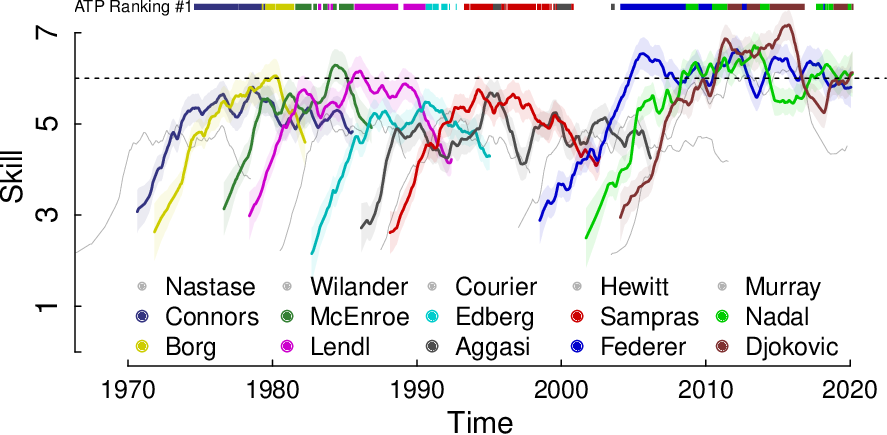
\includegraphics[width=.98\linewidth]{figures/atp}
    \caption{Estimated learning curves for some famous male players. }
    \label{fig:atp}
\end{subfigure}
\caption{\subref{tab:atp_weeks} Historical ranking according to the number of weeks that players reached the first position in the ATP's ranking until March 10, 2020. 
\subref{fig:atp} Estimated skill of some of the historical ATP's leaders. 
The shaded area represents a standard deviation of uncertainty.  
The top bar indicates which player was at the top of the ATP's ranking. 
The dotted line is located at six skill points and helps to compare the curves. 
}
\end{figure}
%
Table~\ref{tab:atp_weeks} shows the historical ranking of players in the top position of the ATP's ranking according to the number of weeks occupying the first position. 
The table is updated to the date of writing this manuscript and, as the ATP's tour was suspended due to COVID-19, 22 weeks are excluded from consideration. 
Figure~\ref{fig:atp} presents the estimated learning curves of some famous male players in ATP's history, which we identified using different colors. 
The top bar indicates which player was at the top of the ATP's ranking (the bar has no color when player number 1 is not considered in our analysis). 

% Parrafo

ATP ranking points are updated every Monday according to the tournament's prestige and the stage reached. 
Only during brief periods, there is no coincidence between the estimated skill and the top player of the ATP's ranking, showing a good agreement between both methodologies. 
Notwithstanding, there are some notorious differences between estimated players' skills and the ATP's ranking, especially concerning the historical ranking shown in Table~\ref{tab:atp_weeks}. 
On the one hand, Lleyton Hewitt's position in the historical ranking is the product of a window of opportunity opened around the year 2000 since his ability is relatively low in historical terms. 
On the other hand, Andy Murray is the fourth most skilled player according to our estimations, but he only reaches 14th place in the historical ranking, just one place above Ilie N\u{a}stase. 

% Parrafo

TrueSkill Through Time allows comparing the relative ability of players over time, unlike historical ATP's ranking and estimators based on the filtering approach (such as TrueSkill).
The learning curves share a similar pattern: they begin with rapid growth, reach an unstable plateau, and end with a slow decline (for visualization purposes, we hide the last portion of the players having long final stages). 
Individual learning curves enable recognition of special periods of crisis and prolonged stability of the professional players, and even the effects of emotional slumps such as those suffered by Aggasi and Djokovic. 
It is worthwhile to note that the skill of tennis players did not increase abruptly over the years: contrary to what is expected, the players of the 1980s were more skilled than those of the 1990s and reached a skill similar to what Federer, Nadal, and Djokovic had in 2020, even though the latter reached higher values for a longer time.

% Parrafo

The previous example summarizes the players' skills using a single dimension. 
TrueSkill Through Time allows estimating multi-dimensional skills. 
It is widely recognized that the ability of certain tennis players varies significantly depending on the surface. 
To quantify this phenomenon, we propose modeling each player as a team composed of a generic player, who is included in all the games, and another player representing the player's ability on a particular surface. 
For example, Nadal is represented by a two-player team: \emph{Nadal\_generic} and \emph{Nadal\_clay} when playing on this kind of surface, and \emph{Nadal\_generic} and \emph{Nadal\_grass} when participating in the Wimbledon tournament. 
%
\begin{lstlisting}[captionpos=b,backgroundcolor=\color{julia!60},label=lst:atp_ground, caption={Modeling multi-dimensional skills in ATP history.}, belowskip=0cm]
players = Set(vcat((composition...)...))
priors = Dict([(p, Player(Gaussian(0., 1.6), 1.0, 0.036) ) for p in players])

composition_ground = [ r.double == "t" ? [[r.w1_id, r.w1_id*r.ground, r.w2_id, r.w2_id*r.ground],[r.l1_id, r.l1_id*r.ground, r.l2_id, r.l2_id*r.ground]] : [[r.w1_id, r.w1_id*r.ground],[r.l1_id, r.l1_id*r.ground]] for r in eachrow(data) ]   

h_ground = History(composition = composition_ground, times = dates, sigma = 1.0, gamma = 0.01, beta = 0.0, priors = priors)
convergence(h_ground, epsilon = 0.01, iterations=10)
\end{lstlisting}
%
In this example, we keep the same prior as in Code~\ref{lst:atp} for all the generic players, but in this code, we define them using the variable \texttt{priors}. 
We create the teams depending on whether the game is double or single, similarly to Code~\ref{lst:atp} but now adding the specific surface skills of each player as their teammate (we use the operator \texttt{*} to concatenate strings). 
As the specific surface skills are not defined in the variable \texttt{prior}, we use the default values defined in the class  \texttt{History} for initialization. 
We also define \texttt{beta} as null for specific surface skills to avoid adding additional noise to the players' performance, keeping the scale of the estimates stable. 
We select a \texttt{sigma} that we consider sufficiently large and a dynamic factor \texttt{gamma} representing \SI{1}{\percent} of the prior uncertainty. 
%
\begin{figure}[ht!]
    \centering
    \begin{subfigure}[t]{0.48\textwidth}
    \includegraphics[page={1},width=\linewidth]{figures/atp_ground}
    \caption{Nadal.}
    \end{subfigure}
    \begin{subfigure}[t]{0.48\textwidth}
    \includegraphics[page={3},width=\linewidth]{figures/atp_ground}
    \caption{Djokovic.}
    \end{subfigure}
    \caption{
    Skill difference on the three main types of surface. 
    Each point on the $y$-axis represents a distance of one $\beta$, i.e.,~\SI{76}{\percent} probability of winning. 
    }
    \label{fig:atp_ground}
\end{figure}

%
% Parrafo
%

In Figure~\ref{fig:atp_ground}, we show the skill difference that Nadal and Djokovic have in each of the three types of ground. 
Nadal has a notorious skill difference when playing on different surfaces. 
On the contrary, Djokovic has very similar skills in the three types. 
The Nadal's skill difference between clay and grass grounds is greater than one $\beta$, which means at least a \SI{76}{\percent} difference in the probability of winning compared to itself. 
In the case of Nadal, it seems important to consider the skill's multi-dimensionality, while in Djokovic's case, it seems reasonable to summarize it in a single dimension. 
To assess whether the complexity added by modeling multi-dimensionality is appropriate in general terms, we can compare the joint prior prediction of the models, calling the method \texttt{log\_evidence()} of the class \texttt{History}. 

%Parrafo

In tennis, it is sufficient to summarize the skills in a single dimension since the prior prediction is maximized when the parameters of the surface's factors (i.e.,~$\sigma$ and $\gamma$) vanish. 
In other examples, where the multi-dimensionality of skills could be more relevant, it should be necessary to model the skills of all agents using different components. 
If we consider only the games in which Nadal participates, optimality is achieved when the parameters take the values $\sigma=0.35$ and $\gamma=0$, meaning that it is necessary to model multidimensional skills ($\sigma>0$) but considering that their effect does not change over time ($\gamma = 0$). 
In this scenario, Nadal's ability on Clay is $0.87\beta$ higher than on Hard and $1.05\beta$ higher than on Grass. 

\section{Models and software} 

This section provides the complete mathematical documentation of the TrueSkill Through Time model. 
The advantage of this model lies in the strict application of probability theory: all the assumptions are made explicit through a generative model, and the inference is solved only with the rules of probability, nothing more than the sum and the product rules. 
Section~\ref{sec:sumProductAlgorithm} introduces the \emph{sum-product algorithm}, which allows us to apply these rules to compute the marginal distributions, e.g., the posterior and the prior prediction. 
Section~\ref{sec:propiedades} lists the properties needed to derive the marginal distributions of interest. 
In Section~\ref{sec:Gaussian}, we introduce the operations of the class \texttt{Gaussian}, which does most of the computation. 
In sections \ref{sec:2vs2}, \ref{sec:empate}, and \ref{sec:approximate_posterior}, we show how to solve the prior prediction and the exact posterior of an event, then we introduce the model for a draw and explain how to approximate the exact posterior in events with two teams. 
Section~\ref{sec:iterative_posterior} explains the general multi-team solution requiring an iterative algorithm. 
Section~\ref{sec:throughTime} justifies the mathematical steps required to solve the full TrueSkill Through Time model. 

\subsection{Sum-product algorithm} \label{sec:sumProductAlgorithm}

The \emph{sum-product algorithm}~\citep{Kschischang2001} takes advantage of the structure of the joint probability distribution imposed by the causal model to apply the probability rules efficiently. 
Any model can be factorized into the product of conditional probabilities. 
Based on the independence between variables, our model (Figure~\ref{fig:generative_model}) can be factorized as,
%
\begin{equation} \label{eq:factorization}
 p(\bm{s},\bm{p},d,r) = p(s_1)p(s_2)p(p_1|s_1)p(p_2|s_2)p(d|\bm{p})P(r|d)
\end{equation}
%
Figure~\ref{fig:factor_graph} shows this factorization graphically. 
These representations, known as \emph{factor graphs}, have two kinds of nodes: variable-type nodes (white circles) and function-type nodes (black squares). 
The edge between node variables and node functions represents the mathematical relationship ``the variable $v$ is an argument of the function $f$''. 
%
\begin{figure}[ht!]
\centering \small
    \tikz{         
%         \node[const, above=of fr] (nfr) {$f_r$}; %
% 	\node[const, above=of nfr] (dfr) {\large $\mathbb{I}(d >0)$}; %
        
    \node[factor] (fr) {} ; 
    \node[const, left=of fr] (nfr) {\normalsize $P(r|d)$}; 
    \node[const, right=of fr] (dfr) {\normalsize \hspace{2.4cm} $P(r|d)=\mathbb{I}(d>0)$}; 

    \node[latent, above=of fr, yshift=-0.6cm] (d) {$d$} ; %
    \node[const, left=of d, xshift=-1.35cm] (d_name) {\small Difference:};
    
    
    \node[factor, above=of d,yshift=-0.6cm] (fd) {} ; 
    \node[const, left=of fd] (nfd) {\normalsize $p(d|\bm{p})$}; 
    \node[const, right=of fd] (dfd) {\normalsize \hspace{2.4cm} $p(d|\bm{p}) =\delta(d=p_1-p_2) $}; 
    
    
    \node[latent, above=of fd, xshift=-0.8cm, yshift=-0.6cm] (p1) {$p_1$} ; %
    \node[latent, above=of fd, xshift=0.8cm, yshift=-0.6cm] (p2) {$p_2$} ; %
    \node[const, left=of p1, xshift=-0.55cm] (p_name) {\small Performance:}; 

    \node[factor, above=of p1 ,yshift=-0.6cm] (fp1) {} ; 
    \node[factor, above=of p2 ,yshift=-0.6cm] (fp2) {} ; 
    
    \node[latent, above=of fp1,yshift=-0.6cm] (s1) {$s_1$} ; %
    \node[latent, above=of fp2,yshift=-0.6cm] (s2) {$s_2$} ; %
    
    \node[factor, above=of s1 ,yshift=-0.6cm] (fs1) {} ; 
    \node[factor, above=of s2 ,yshift=-0.6cm] (fs2) {} ; 
    
    
    \node[const, left=of fp1] (nfp1) {\normalsize $p(p_1|s_1)$};
    \node[const, right=of fp2] (nfp2) {\normalsize $p(p_2|s_2)$};
    \node[const, right=of fp2] (dfp2) {\normalsize \hspace{1.6cm} $p(p_i|s_i)=\N(p_i|s_i,\beta^2)$};

    \node[const, left=of s1, xshift=-.85cm] (s_name) {\small Skill:}; 
    
    \node[const, left=of fs1] (nfs1) {\normalsize $p(s_1)$};
    \node[const, right=of fs2] (nfs2) {\normalsize $p(s_2)$};
    \node[const, right=of fs2] (dfs) {\normalsize \hspace{1.6cm} $p(s_i) = \N(s_i|\mu_i,\sigma_i^2)$};

    
    \edge[-] {d} {fr};
    \edge[-] {p1,p2,d} {fd};
    \edge[-] {fp1} {p1,s1};
    \edge[-] {fp2} {p2,s2};
    \edge[-] {fs1} {s1};
    \edge[-] {fs2} {s2};
}
     \caption{%
     Graphical way of representing the joint distribution factorization induced by the basic causal model, represented by Equation~\ref{eq:factorization}. 
     Black squares represent the functions, white circles represent the variables, and the edges between them represent the mathematical relationship ``the variable is the argument of the function''. 
     }
    \label{fig:factor_graph}
\end{figure} 
%
In our case, we want to compute two marginals, the proportional posterior of the skills $p(s_i, r)$ and the prior probability of the result $p(r)$. 
The \emph{sum-product algorithm} is a general way of breaking down the rules of probability as messages sent between the nodes of the \emph{factor graph}. 
There are two types of messages: those sent by variable-type nodes to their function-type neighbors ($m_{v \rightarrow f}(v)$) and the ones that function-type nodes send to their variable-type neighbors ($m_{f \rightarrow v}(v)$). 
The former partially performs the product rule. 
%
\begin{equation*}\label{eq:m_v_f} \tag{\text{product step}}
m_{v \rightarrow f}(v) = \prod_{h \in n(v) \setminus \{f\} } m_{h \rightarrow v}(v)
\end{equation*}
%
where $n(v)$ represents the set of neighbor nodes to $v$. 
In brief, the messages sent by the variable-type node $v$ are the product of the messages that $v$ receives from the rest of their neighbors $h \in n(v)$ except $f$. 
The messages sent by the function-type nodes encode a portion of the sum rule. 
%
\begin{equation*}\label{eq:m_f_v}  \tag{\text{sum step}}
m_{f \rightarrow v}(v) = \int \cdots \int \Big( f(\bm{h},v) \prod_{h \in n(f) \setminus \{v\} } m_{h \rightarrow f}(h) \Big) \,  d\bm{h}
\end{equation*}
%
where $\bm{h} = n(f)\setminus \{v\}$ is the set of all neighbors to $f$ except $v$, and $f(\bm{h},v)$ represents the function $f$, evaluated in all its arguments. 
In brief, the messages sent by a function $f$ are also the product of the messages it receives from the rest of its neighbors $h \in n(f)$ except $v$, but this time it is also multiplied by itself $f(\cdot)$ and integrated (or summed) over $\bm{h}$. 
Finally, the marginal probability distribution of a variable $v$ is simply the product of the messages that $v$ receives from all its neighbors. 
%
\begin{equation*}\label{eq:marginal}  \tag{\text{marginal probability}}
p(v) = \prod_{h \in n(v)} m_{h \rightarrow v}
\end{equation*}
%
This algorithm encodes the minimum number of steps required to calculate any marginal probability distribution. 

\subsection{Mathematical properties and notation}\label{sec:propiedades}

The efficiency of TrueSkill Through Time is based on the analytical computation of marginal probabilities. 
This section lists the needed properties to derive the exact and approximate messages generated by the sum-product algorithm.  
The first property states that the product of two Gaussian distributions evaluated at the same point $x$ can be expressed as the product of two other Gaussian distributions with only one evaluated at $x$. 
%
\begin{equation*}\label{eq:gaussian_product} \tag{\text{Gaussian product}}
\N(x|\mu_1,\sigma_1^2)\N(x|\mu_2,\sigma_2^2) \overset{\ref{multiplicacion_normales}}{=} \N(\mu_1|\mu_2,\sigma_1^2+\sigma_2^2) \N(x|\mu_{*},\sigma_{*}^2)
\end{equation*}
%
where $\mu_{*} = \frac{\mu_1}{\sigma_1^2} + \frac{\mu_2}{\sigma_2^2}$ y $\sigma_{*}^2 = \left(\frac{1}{\sigma_1^2} + \frac{1}{\sigma_2^2} \right)^{-1}$.
Something similar occurs with the division of two Gaussian distributions, both evaluated at the same point $x$. 
%
\begin{equation*}\label{eq:gaussian_division} \tag{\text{Gaussian division}}
\N(x|\mu_1,\sigma_1^2)/\N(x|\mu_2,\sigma_2^2) \overset{\ref{sec:division_normales}}{\propto} \N(x|\mu_{\div},\sigma_{\div}^2)/\N(\mu_1|\mu_2,\sigma_1^2+\sigma_2^2) 
\end{equation*}
%
where $\mu_{\div} = \frac{\mu_1}{\sigma_1^2} - \frac{\mu_2}{\sigma_2^2}$ y $\sigma_{\div}^2 = \left(\frac{1}{\sigma_1^2} - \frac{1}{\sigma_2^2} \right)^{-1}$.

%
% Parrafo
%

The indicator function $\mathbb{I}(\cdot=\cdot)$ is $1$ when equality is true and $0$ otherwise. 
It represents probabilities distributions of non-random discrete variables, such as the result of the games given the difference of performances $p(r|d)$. 
Similarly, the Dirac delta function $\delta(\cdot=\cdot)$ represents probabilities distributions of non-random continuous variables, such as the difference of performances given the agents' performances $p(d|\bm{p})$. 
If we can use it to replace a variable within an integral,
%
\begin{equation*}\label{eq:integral_con_dirac} \tag{\text{Dirac delta function}}
\begin{split}
 \iint  \delta(x=h(y,z)) f(x) g(y)\, dx\, dy = \int f(h(y,z)) g(y) dy
 \end{split}
\end{equation*}
the dimensionality of the problem is reduced. 
We also use the properties derived from the symmetry of Gaussian distributions. 
\begin{equation*}\label{eq:simetria} \tag{\text{Gaussian symmetry}}
 \N(x|\mu,\sigma^2) = \N(\mu|x,\sigma^2) = \N(-\mu|-x,\sigma^2) = \N(-x|-\mu,\sigma^2) 
\end{equation*}
The Gaussian standardization,
\begin{equation*}\label{eq:estandarizar} \tag{\text{Gaussian standardization}}
  \N(x|\mu,\sigma^2) = \N((x-\mu)/\sigma | 0, 1)
\end{equation*}
Equality between the Gaussian distribution and the derivative of their cumulative distribution,
\begin{equation*}\label{eq:phi_norm} \tag{\text{Derivative of the cumulative Gaussian}}
\frac{\partial}{\partial x} \Phi(x|\mu,\sigma^2) = \N(x|\mu,\sigma^2)
\end{equation*}
%
which is valid by definition. 
The symmetry of the cumulative Gaussian distribution. 
%
\begin{equation*}\label{eq:phi_simetria} \tag{\text{Symmetry of the cumulative Gaussian}}
\Phi(0|\mu,\sigma^2) = 1-\Phi(0|-\mu,\sigma^2)
\end{equation*}

\subsection{The Gaussian class}\label{sec:Gaussian}

The \texttt{Gaussian} class does most of the computation of the packages. 
It is characterized by the mean (\texttt{mu}) and the standard deviation (\texttt{sigma}). 
%
\begin{lstlisting}[captionpos=b,backgroundcolor=\color{all},label=lst:N1_N2, caption={Initialization of Gaussian distributions.}, belowskip=0cm]
N1 = Gaussian(mu = 1.0, sigma = 1.0); N2 = Gaussian(1.0, 2.0)  
\end{lstlisting}
The class overwrites the addition (\texttt{+}), subtraction (\texttt{-}), product (\texttt{*}), and division (\texttt{/}) to compute the marginal distributions used in the TrueSkill Through Time model. 
%
\begin{equation*} \tag{\texttt{N1 * N2}}
 \N(x|\mu_1,\sigma_1^2)\N(x|\mu_2,\sigma_2^2) \overset{\ref{multiplicacion_normales}}{\propto} \N(x|\mu_{*},\sigma_{*}^2)
\end{equation*}
%
\begin{equation*} \tag{\texttt{N1 / N2}}
 \N(x|\mu_1,\sigma_1^2)/\N(x|\mu_2,\sigma_2^2)  \overset{\ref{sec:division_normales}}{\propto} \N(x|\mu_{\div},\sigma_{\div}^2)
\end{equation*} 
%
\vspace{-0.3cm}
%
\begin{equation*} \tag{\texttt{N1 + N2}} \label{eq:suma_normales}
\begin{split}
\iint \delta(t=x + y) \N(x|\mu_1, \sigma_1^2)\N(y|\mu_2, \sigma_2^2) dxdy \overset{\text{\ref{suma_normales_induccion}}}{=} \N(t|\mu_1+\mu_2,\sigma_1^2 + \sigma_2^2)
\end{split}
\end{equation*}
%
\vspace{-0.5cm}
%
\begin{equation*} \tag{\texttt{N1 - N2}} \label{eq:resta_normales}
\begin{split}
\iint \delta(t = x - y) \N(x|\mu_1, \sigma_1^2)\N(y|\mu_2, \sigma_2^2) dxdy \overset{\text{\ref{suma_normales_induccion}}}{=} \N(t|\mu_1 - \mu_2,\sigma_1^2 + \sigma_2^2)
\end{split}
\end{equation*}
%
Although these properties are widely known, we attach their complete demonstrations in the supplemental material. 

\subsection{The exact solution for events with two teams}\label{sec:2vs2}

In the presence of teams, the Elo model assumes that a team's performance is the sum of the performance of its members. The team with the highest performance wins, $r = (t_i> t_j)$. 
Figure~\ref{fig:modelo_trueskill_2vs2} shows the graphical factorization of the Elo team model. 
%
\begin{figure}[ht!]
  \centering
  \scalebox{.9}{
  \tikz{
      
        \node[factor] (fr) {} ;
        \node[const, right=of fr] (nfr) {$f_{r}$}; %
	
	\node[latent, above=of fr, yshift=-0.4cm] (d) {$d$} ; %
        \node[factor, above=of d, yshift=-0.4cm] (fd) {} ;
        \node[const, above=of fd] (nfd) {$f_{d}$}; %
	
        
        \node[latent, left=of fd,xshift=0.4cm] (ta) {$t_a$} ; %
        \node[factor, left=of ta,xshift=0.4cm] (fta) {} ;
        \node[const, above=of fta] (nfta) {$f_{t_a}$}; %
        
        \node[latent, left=of fta,yshift=1cm,xshift=0.4cm] (p1) {$p_1$} ; %
        \node[factor, left=of p1,xshift=0.4cm] (fp1) {} ;
        \node[const, above=of fp1] (nfp1) {$f_{p_1}$}; %
        
        \node[latent, left=of fp1,xshift=0.4cm] (s1) {$s_1$} ; %
        \node[factor, left=of s1,xshift=0.4cm] (fs1) {} ;
	\node[const, above=of fs1] (nfs1) {$f_{s_1}$}; %
     
        \node[latent, left=of fta,yshift=-1cm,xshift=0.4cm] (p2) {$p_2$} ; %
        \node[factor, left=of p2,xshift=0.4cm] (fp2) {} ;
        \node[const, above=of fp2] (nfp2) {$f_{p_2}$}; %
        
        \node[latent, left=of fp2,xshift=0.4cm] (s2) {$s_2$} ; %
        \node[factor, left=of s2,xshift=0.4cm] (fs2) {} ;
	\node[const, above=of fs2] (nfs2) {$f_{s_2}$}; %
        
            
        \node[latent, right=of fd,xshift=-0.4cm] (tb) {$t_b$} ; %
        \node[factor, right=of tb,xshift=-0.4cm] (ftb) {} ;
        \node[const, above=of ftb] (nftb) {$f_{t_b}$}; %
        
        \node[latent, right=of ftb,yshift=1cm,xshift=-0.4cm] (p3) {$p_3$} ; %
        \node[factor, right=of p3,xshift=-0.4cm] (fp3) {} ;
        \node[const, above=of fp3] (nfp3) {$f_{p_3}$}; %
        
        \node[latent, right=of fp3,xshift=-0.4cm] (s3) {$s_3$} ; %
        \node[factor, right=of s3,xshift=-0.4cm] (fs3) {} ;
	\node[const, above=of fs3] (nfs3) {$f_{s_3}$}; %
     
        \node[latent, right=of ftb,yshift=-1cm,xshift=-0.5cm] (p4) {$p_4$} ; %
        \node[factor, right=of p4,xshift=-0.4cm] (fp4) {} ;
        \node[const, above=of fp4] (nfp4) {$f_{p_4}$}; %
        
        \node[latent, right=of fp4,xshift=-0.4cm] (s4) {$s_4$} ; %
        \node[factor, right=of s4,xshift=-0.4cm] (fs4) {} ;
	\node[const, above=of fs4] (nfs4) {$f_{s_4}$}; %
     
        \edge[-] {fr} {d};
	\edge[-] {d} {fd};
	
        \edge[-] {fd} {ta};
        \edge[-] {ta} {fta};
        \edge[-] {fta} {p1};
        \edge[-] {p1} {fp1};
        \edge[-] {fp1} {s1};
        \edge[-] {s1} {fs1};
        \edge[-] {fta} {p2};
        \edge[-] {p2} {fp2};
        \edge[-] {fp2} {s2};
        \edge[-] {s2} {fs2};
        	
	\edge[-] {fd} {tb};
        \edge[-] {tb} {ftb};
        \edge[-] {ftb} {p3};
        \edge[-] {p3} {fp3};
        \edge[-] {fp3} {s3};
        \edge[-] {s3} {fs3};
        \edge[-] {ftb} {p4};
        \edge[-] {p4} {fp4};
        \edge[-] {fp4} {s4};
        \edge[-] {s4} {fs4};
        
	
	\node[const, below=of fr,xshift=7cm,yshift=-0.3cm] (dfr) { $f_r = \mathbb{I}(d>0)$}; %
	\node[const, left=of dfr,xshift=-0.5cm] (dfd) {$f_d = \delta(d=t_a - t_b)$}; %
	\node[const, left=of dfd,xshift=-0.5cm] (dft) {$f_{t_e} = \delta(t_e = \sum_{i \in A_e} p_i)$}; %
        \node[const, left=of dft,xshift=-0.5cm] (dfp) {$f_{p_i} = \N(p_i|s_i,\beta^2)$}; %
        \node[const, left=of dfp,xshift=-0.5cm] (dfs) {$f_{s_i} = \N(s_i|\mu_i,\sigma^2)$}; %
   }
   }
  \caption{Factor graph of a game with two teams with two players each. 
  The Elo's team model incorporate a new variable, $t$, that models the team performance.}
  \label{fig:modelo_trueskill_2vs2}
\end{figure}
%
In this example, we have two teams with two players each. 
Every two-teams game has an analytical solution. 

% Parrafo

This section shows the steps to compute the exact evidence and likelihoods for a game with two teams. 
We only need the \emph{sum-product algorithm} and the properties mentioned above. 
We will start first with the ``descending'' messages from the priors to the result until computing the evidence. 
Then, we continue with the ``ascending'' messages from the observed result and to the priors until computing each agent's posterior. 

\paragraph{Descending messages.}
%
Following the \ref{eq:m_f_v} of the sum-product algorithm and the factorization of the model displayed in Fig.~\ref{fig:modelo_trueskill_2vs2}, messages sent by the skill factors $f_{s_i}$ to the variable $s_i$ are just the priors. 
%
\begin{equation*}\label{eq:m_fs_s} \tag{\texttt{prior}}
 m_{f_{s_i} \rightarrow s_i}(s_i) = \N(s_i| \mu_i, \sigma_i^2)
\end{equation*}
%
We have access to this message by calling the \texttt{prior} attribute of the \texttt{Player} class. 
Following the~\ref{eq:m_v_f} of the sum-product algorithm and the factorization of the model, the message sent by the variable $s_i$ to the performance factor $f_{p_i}$ is the prior. 
Since it is trivial to calculate the messages sent by the variables (they are the product of the messages received from behind), we do not include them. 
Then, the message sent by the performance factors $f_{p_i}$ to the variable $p_i$ is: 
%
\begin{equation*}\label{eq:m_fp_p} \tag{\texttt{performance()}}
m_{f_{p_i} \rightarrow p_i}(p_i) = \int \N(p_i| s_i, \beta^2) \N(s_i| \mu_i, \sigma_i^2) ds_i = \N(p_i|\mu_i,\beta^2 + \sigma_i^2)
\end{equation*}
%
We have access to these messages through the \texttt{performance()} method of the \texttt{Player} class. 
%
\begin{paracol}{3}
\begin{lstlisting}[backgroundcolor=\color{julia!60},belowskip=0cm]
p1 = performance(a1)
p2 = performance(a2)
p3 = performance(a3)
p4 = performance(a4)
\end{lstlisting}
  \switchcolumn
\begin{lstlisting}[backgroundcolor=\color{python!60},belowskip=0cm]
p1 = a1.performance()
p2 = a2.performance()
p3 = a3.performance()
p4 = a4.performance()
\end{lstlisting}
   \switchcolumn
\begin{lstlisting}[backgroundcolor=\color{r!50},belowskip=0cm]
p1 = performance(a1)
p2 = performance(a2)
p3 = performance(a3)
p4 = performance(a4)
\end{lstlisting}  
\end{paracol}
\begin{lstlisting}[captionpos=b,backgroundcolor=\color{white},label=lst:performance, caption={Computing the individual prior performance.}, aboveskip=0cm, belowskip=0cm]
\end{lstlisting}
where the agents \texttt{a1}, \texttt{a2}, \texttt{a3}, and \texttt{a4} were initialized in Code~\ref{lst:player}. 
The message sent by the team factors $f_{t_e}$ to the team variable $t_e$ is an integral over all the individual performance variables,
\begin{equation*} \label{eq:m_ft_t} \tag{\texttt{ta = p1 + p2}}
\begin{split}
 m_{f_{t_e} \rightarrow t_e}(t_e) &= \iint \delta(t_e = p_i + p_j) \N(p_i|\mu_i,\beta^2 + \sigma_i^2)\N(p_j|\mu_j,\beta^2 + \sigma_j^2) dp_idp_j  \\ &=  \N(t_e|\underbrace{\mu_i+\mu_j}_{\text{\normalsize $\mu_e\phantom{^2}$}}, \underbrace{2\beta^2 + \sigma_i^2 + \sigma_j^2}_{\text{\normalsize $\sigma_e^2$}})
\end{split}
\end{equation*}
where the Dirac delta function imposes the constraint that the sum of the individual performances equals a constant team performance value $t_e$. 
Applying the already presented properties, we can solve this integral analytically, obtaining the prior performance of the teams, which is a Gaussian distribution centered on the sum of the mean estimates $\mu_e = \mu_i + \mu_j$ with a variance $\sigma_e^2$ including both the uncertainties of the estimates (i.e.,~$\sigma_i^2 + \sigma_j^2$) and the variance of the individual performances (i.e.,~2$\beta^2$). 
We have access to this message using the operator \texttt{+} of the class \texttt{Gaussian} to sum the agents' performances,
\begin{lstlisting}[captionpos=b,backgroundcolor=\color{all},label=lst:team_performance, caption={Computing the team prior performance.}, belowskip=0cm]
ta = p1 + p2; tb = p3 + p4
\end{lstlisting}
%
The next message, sent by the difference factor $f_{d_1}$ to the difference variable $d_1$, is:
\begin{equation*}\label{eq:m_fd_d} \tag{\texttt{d = ta - tb}}
 \begin{split} 
  m_{f_{d} \rightarrow d}(d) & = \iint \delta(d = t_a - t_b) \N(t_a| \mu_a, \sigma_a^2)  \N(t_b| \mu_b, \sigma_b^2)  dt_adt_b \\[0.25cm]
  & = \N\big( d | \underbrace{\mu_a - \mu_b}_{\hfrac{\text{Expected difference}}:  \ \psi}, \underbrace{\sigma_a^2 +\sigma_b^2}_{\hfrac{\text{Total}}{\text{uncertainty}} : \ \vartheta^2}  \big) = \N(d | \psi, \, \vartheta^2)
 \end{split}
\end{equation*}
%
The prior difference of performance is a Gaussian distribution centered on the prior expected difference between teams $\psi = \mu_a - \mu_b$ with variance $\vartheta^2 = \sigma_a^2 + \sigma_b^2$ that includes the uncertainty of both teams. 
We have access to this message using the operator \texttt{-} of the class \texttt{Gaussian} to get the difference of teams' performances,
%
\begin{lstlisting}[captionpos=b,backgroundcolor=\color{all},label=lst:difference_performance, caption={Computing the prior perfomance' difference}, belowskip=0cm]
d = ta - tb 
\end{lstlisting}
%
The last descending message, sent by the factor $f_r$ to the variable $r$, allows to compute the evidence, i.e.,~the prior prediction of the observed result. 
%
\begin{equation*}\label{eq:m_fr_r} \tag{\texttt{evidence}}
\begin{split}
 m_{f_{r} \rightarrow r}(r) = \int \mathbb{I}(d > 0) \N(d | \psi, \vartheta^2)  dd = 1 - \Phi(0|\psi, \vartheta^2)
\end{split}
\end{equation*}
%
We have access to this message by computing the cumulative value from $0$ to $\infty$ of the team difference of performances distribution. 
%
\begin{paracol}{3}
\begin{lstlisting}[backgroundcolor=\color{julia!60}, belowskip=0cm]
e = 1.0 - cdf(d, 0.0)
\end{lstlisting}  
 \switchcolumn
\begin{lstlisting}[backgroundcolor=\color{python!60}, belowskip=0cm]
e = 1 - cdf(0,d.mu,d.sigma) 
\end{lstlisting} 
 \switchcolumn
\begin{lstlisting}[backgroundcolor=\color{r!50}, belowskip=0cm]
e = 1 - cdf(0,d@mu,d@sigma) 
\end{lstlisting}
\end{paracol}
\begin{lstlisting}[captionpos=b,backgroundcolor=\color{white},label=lst:difference, caption={Computing the prior prediction of the observed result (or evidence).}, aboveskip=0cm, belowskip=0cm]
\end{lstlisting}
%
where \texttt{e} contains the value of equation \texttt{evidence}. 

\paragraph{Ascending messages.}
%
Now, we examine the ascending messages. 
The result factor $f_r$ sends to the difference variable $d$ the first ascending message. 
%
\begin{equation}%\label{eq:m_fr_d} \tag{\texttt{exact\_lhood\_d}}
\begin{split}
m_{f_r \rightarrow d}(d) & = \mathbb{I}(d>0)
\end{split}
\end{equation}
%
This message contains the indicator function of the factor $f_r$ that transmits the information of the observed result. 
The message sent by difference factor $f_d$ to the winning team performance variables $t_e$ is:
%
\begin{equation}%\label{eq:m_fd_ta} \tag{\texttt{exact\_lhood\_ta}}
\begin{split}
m_{f_{d} \rightarrow t_a}(t_a) & = \iint \delta(d = t_a - t_b) \mathbb{I}(d > 0) \N(t_b | \mu_b , \sigma_b^2 ) \, dd\,dt_b \\
& = \int \mathbb{I}( t_a > t_b)  \N(t_b | \mu_b , \sigma_b^2 ) \,dt_b  = 1 - \Phi (0| t_a -\mu_b, \sigma_b^2) = \Phi (t_a| \mu_b, \sigma_b^2)
\end{split}
\end{equation}
%
In this case, the previous upstream message is integrated with the downstream message from the other team. 
This message, parametrized at $t_a$, is the cumulative of the Gaussian distribution of the opposing team's performances from $t_a$ to $\infty$, and encodes the likelihood of the winning team performance hypotheses. 
The message sent by team performance factor $f_{t_a}$ to the variable of the individual performance $p_1$ is:
%
\begin{equation}%\label{eq:m_fta_p_inicial} \tag{\texttt{exact\_lhood\_p1}}
\begin{split}
m_{f_{t_a} \rightarrow p_1}(p_1)  & = \iint \delta( t_a = p_1 + p_2) \, N(p_2| \mu_2, \beta^2 + \sigma_2^2 ) \, \Phi (t_a| \mu_b , \sigma_b^2 ) \, dt_a dp_2 \\
& = \int  \, \N(p_2| \mu_2, \beta^2 + \sigma_2^2 ) \, \Phi (p_1 + p_2| \mu_b , \sigma_b^2 ) \, dp_2 \\
& = 1 - \Phi( 0 | p_1 + \underbrace{\mu_2 - \mu_b}_{\mu_1 - \psi}, \underbrace{\beta^2 + \sigma_2^2 + \sigma_b^2}_{\vartheta^2 - (\sigma_1^2 + \beta^2)}) \\
\end{split}
\end{equation}
%
Again, the previous upstream message is integrated with a downstream message, the prior performance of their teammate. 
The message, parameterized at $p1$, encodes the likelihood of the individual performance hypotheses of the winning player. 
The last message, sent by individual performance factor $f_{p_1}$ to the skill variable $s_1$ is:
%
\begin{equation}%\label{eq:m_fp_s1} \tag{\texttt{exact\_lhood\_s1}}
\begin{split}
m_{f_{p_1} \rightarrow s_1}(s_1) & = \int N(p_1| s_1, \beta^2) \, \Phi(p_1| \mu_1-\psi, \vartheta^2 - (\sigma_1^2 + \beta^2)) \, dp_1 \\[0.1cm]
& = 1 - \Phi(0 | \underbrace{(s_1 + \mu_2) - (\mu_3 + \mu_4)}_{\hfrac{\text{Expected difference}}{\text{parameterized in $s_1$}} } \ , \underbrace{\ \ \ \ \vartheta^2 - \sigma_1^2 \ \ \ \ }_{\hfrac{\text{Total uncertainty}}{\text{except the one of $s_1$}}})\end{split}
\end{equation}
%
This corresponds to the exact likelihood presented in Equation~\ref{eq:posterior_win}, which computes the prior probability of winning result if the player's actual skill was $s_1$. 

\subsection{A basic model for a draw} \label{sec:empate}

The model for a draw assumes that a tie occurs when the difference in performance does not exceed a threshold, $|t_a - t_b| \leq \varepsilon$. 
In Figure~\ref{fig:draw_a}, we graphically display the probabilities of the three possible outcomes. 
%
\begin{figure}[ht!]
\centering
\begin{subfigure}[t]{0.48\textwidth}
  \includegraphics[width=1\textwidth]{figures/draw.pdf} 
  \caption{The three possible results.}
  \label{fig:draw_a}
\end{subfigure}
\begin{subfigure}[t]{0.48\textwidth}
  \includegraphics[page=2,width=1\textwidth]{figures/draw.pdf}
  \caption{Constant draw probability.}
  \label{fig:draw_b}
\end{subfigure}
\caption{Distribution of performance difference under the draw model. 
\subref{fig:draw_a}: example of the areas corresponding to the probability of losing, drawing and winning. 
\subref{fig:draw_b} shows how the tie margin should be adapted to keep the tie probability constant when the uncertainty of the distribution changes. 
}
\label{fig:draw}
\end{figure}

%
% Parrafo
%

This model requires establishing the threshold for considering a draw. 
Herbrich et al.~\citep{Herbrich2007} propose using the empirical frequency of ties to define it. 
However, this value depends on the actual skill difference, which is unknown. 
Assuming that we can define the ``probability of a draw between teams with the same skill'' then the threshold also depends on the number of players. 
Figure~\ref{fig:draw_b} shows that to keep the tie area constant, it is necessary to adapt the threshold according to the uncertainty. 
Since the observed results are independent of our beliefs, the only source of uncertainty is the variance of individual performance $\beta$. 
Then, we can define an expression that links the threshold $\varepsilon$ with the probability of a tie: 
%
\begin{equation}
 \text{Draw probability} = \Phi(\frac{\varepsilon}{\sqrt{n_1+n_2}\beta}) - \Phi(\frac{-\varepsilon}{\sqrt{n_1+n_2}\beta})
\end{equation}
%
In the Code~\ref{lst:draw}, we use the function \texttt{compute\_margin()} to get the size of the margin. 

\begin{paracol}{3}
\begin{lstlisting}[backgroundcolor=\color{julia!60},belowskip=0cm]
na = length(team_a)
nb = length(team_b)
sd = sqrt(na + nb)*beta
\end{lstlisting}
\switchcolumn
\begin{lstlisting}[backgroundcolor=\color{python!60},belowskip=0cm]
na = len(team_a)
nb = len(team_b)
sd = math.sqrt(na + nb)*beta
\end{lstlisting}
\switchcolumn
\begin{lstlisting}[backgroundcolor=\color{r!50},belowskip=0cm]
na = length([a1, a2])
nb = length([a3, a4])
sd = sqrt(na + nb)*beta
\end{lstlisting}
\end{paracol}
\begin{lstlisting}[captionpos=b,backgroundcolor=\color{all},label=lst:draw, caption={Computing the draw margin.}, aboveskip=0cm, belowskip=0cm]
p_draw = 0.25
margin = compute_margin(p_draw, sd)
\end{lstlisting}
%
where the individual agents (\texttt{a1} to \texttt{a4}) were initialized in Code~\ref{lst:player} and \texttt{beta} in Code~\ref{lst:parameters}. 


\subsection{Optimal approximation of the exact posterior} \label{sec:approximate_posterior}

In Section~\ref{sec:2vs2}, we presented the procedure to obtain the exact posterior. 
In this section, we show how to obtain the Gaussian distribution that best approximates the exact posterior, considering the possibility of ties. 
The packages solve it with the two lines of Code~\ref{lst:post_2vs2}. 
%
\begin{lstlisting}[backgroundcolor=\color{all},belowskip=-0.77 \baselineskip]
g = Game(teams, p_draw = 0.25)
\end{lstlisting}  
\begin{paracol}{3}
\begin{lstlisting}[backgroundcolor=\color{julia!60}, belowskip=0cm]
post = posteriors(g)
\end{lstlisting}
\switchcolumn
\begin{lstlisting}[backgroundcolor=\color{python!60}, belowskip=0cm]
post = g.posteriors()
\end{lstlisting}
\switchcolumn
\begin{lstlisting}[backgroundcolor=\color{r!50}, belowskip=0cm]
post = posteriors(g)
\end{lstlisting}
\end{paracol}
\begin{lstlisting}[captionpos=b,backgroundcolor=\color{white}, label=lst:post_2vs2, caption={Computing the approximate posterior.}, belowskip=0cm, aboveskip=0cm]
\end{lstlisting}
%
where the variable \texttt{teams} was initialized in Code~\ref{lst:game}. 
The need to approximate the posterior occurs because the distribution of the difference of performances is a truncated Gaussian. 
%
\begin{equation}\label{eq:p_d}
p(d) =
\begin{cases}
\N(d|\psi,\vartheta^2) \mathbb{I}(-\varepsilon < d < \varepsilon) & \text{tie} \\
\N(d|\psi,\vartheta^2) \mathbb{I}(d > \varepsilon) & \text{not tie}
\end{cases}
\end{equation}
%
It is known that the exponential family, to which the Gaussian distribution belongs, minimizes the Kullback-Leibler divergence with respect to the true distribution $p$, $KL(p||q)$ when both have the same moments~\citep{Minka2005}. 
The expectation and variance of a truncated Gaussian $\N(x|\mu,\sigma^2)$ in the range from $a$ to $b$ are:
%
\begin{equation}\label{eq:mean_aprox_double}
 E(X| a < X < b) = \mu + \sigma \frac{\N(\alpha) - \N(\beta) }{\Phi(\beta) - \Phi(\alpha) }
\end{equation}
%
\begin{equation}\label{eq:variance_aprox_double}
 V(X| a < X < b) = \sigma^2 \Bigg( 1 + \bigg(\frac{\alpha N(\alpha) - \beta N(\beta) }{\Phi(\beta) - \Phi(\alpha) }\bigg) - \bigg(\frac{N(\alpha) - N(\beta) }{\Phi(\beta) - \Phi(\alpha) }\bigg)^2 \Bigg)
\end{equation}
where $\beta = \frac{b-\mu}{\sigma}$ and $\alpha = \frac{a-\mu}{\sigma}$. 
With a single-sided truncation, they can be simplified as:
\begin{equation*}
 E(X| a < X )   =  \mu + \sigma \frac{\N(\alpha)}{1 - \Phi(\alpha) } \ \ , \ \ V(X| a < X )  = \sigma^2 \Bigg( 1 + \bigg(\frac{\alpha \N(\alpha)}{1 - \Phi(\alpha) }\bigg) - \bigg(\frac{\N(\alpha)}{1 - \Phi(\alpha) }\bigg)^2 \Bigg) 
\end{equation*}
%
Then, the Gaussian that best approximates $p(d)$ is:
%
\begin{equation}\label{eq:p*_d} \tag{\texttt{approx()}}
 \widehat{p}(d) = \N(d | \widehat{\psi}, \widehat{\vartheta}^2) =
 \begin{cases*}
 \N\Big(d \,  | \, E(d | -\varepsilon < d < \varepsilon ) , \,  V(d | -\varepsilon < d < \varepsilon ) \, \Big) & \text{tie} \\
\N\Big(d \,  | \, E(d | d > -\varepsilon ) , \,  V(d | d > -\varepsilon ) \, \Big) & \text{not tie}
  \end{cases*}
\end{equation}
%
\begin{paracol}{3}
\begin{lstlisting}[backgroundcolor=\color{julia!60},belowskip=0cm]
tie = true
\end{lstlisting}
\switchcolumn
\begin{lstlisting}[backgroundcolor=\color{python!60},belowskip=0cm]
tie = True
\end{lstlisting}
\switchcolumn
\begin{lstlisting}[backgroundcolor=\color{r!50},belowskip=0cm]
tie = T
\end{lstlisting}
\end{paracol}
\begin{lstlisting}[captionpos=b,backgroundcolor=\color{all},label=lst:d_approx, caption={Computing the approximation of the performance difference.},belowskip=0cm,aboveskip=0cm]
d_approx = approx(d, margin, !tie)
\end{lstlisting}
%
where the difference distribution \texttt{d} was initialized in Code~\ref{lst:difference_performance} and the variable \texttt{margin} in Code~\ref{lst:draw}. 
Given $\widehat{p}(d)$, we can compute the approximate ascending message using the methods of the \texttt{Gaussian} class. 
To derive the first ascending message, recall that any marginal distribution can be calculated as the product of the messages received from all its neighboring factors. 
%
\begin{equation}\label{eq:m^_d_fd} \tag{\texttt{approx\_lh\_d}}
\begin{split}
 m_{d \rightarrow f_{d}}(d)   = \frac{p(d)}{m_{f_{d} \rightarrow d}(d)} 
 & \approx \frac{\widehat{p}(d)}{m_{f_{d} \rightarrow d}(d)}  \\
& = \frac{\N(d \,  | \,\widehat{\psi} , \, \widehat{\vartheta}^{\,2} )}{\N(d | \psi, \vartheta^2)} 
\propto N(d,\psi_{\div},\vartheta_{\div}^2 )
\end{split}
\end{equation}
where $m_{f_r \rightarrow d}(d) = m_{d \rightarrow f_{d}}(d)$ holds due to the factorization of the model. 
We have access to this message when we use the \texttt{/} operator of the \texttt{Gaussian} class to divide the distributions:
%
\begin{lstlisting}[captionpos=b,backgroundcolor=\color{all},label=lst:d_div, caption={Computing the first approximate message.},belowskip=0cm]
approx_lh_d = d_approx / d
\end{lstlisting}
All these approximate messages can be interpreted as likelihoods because they transmit the information of the observed result. 
The approximate message sent by difference factor $f_d$ to the winning team performance variables $t_a$ is:
\begin{equation}%\label{eq:^m_fd_ta} \tag{\texttt{approx\_lhood\_ta}}
\begin{split}
\widehat{m}_{f_{d} \rightarrow t_a}(t_a) & =  \iint \delta(d = t_a - t_b) \N(d_1 | \psi_{\div}, \vartheta_{\div}^2) \N(t_b | \mu_b , \sigma_b^2 )  \, d{d} \,dt_b \\
& = \int  \N( t_a-t_b | \psi_{\div}, \vartheta_{\div}^2) \N(t_b | \mu_b , \sigma_b^2 )  \,  d_{t_b} = \N(t_a \, | \, \mu_b + \psi_{\div} \, , \, \vartheta_{\div}^2 + \sigma_b^2) \\
\end{split}
\end{equation}
%
The approximate message sent by team performance factor $f_{t_a}$ to the winning individual performance variables $p_1$ is:%
%
\begin{equation}%\label{eq:^m_fta_p} \tag{\texttt{lhood\_p1\_approx}}
\begin{split}
\widehat{m}_{f_{t_a} \rightarrow p_1}(p_1) &= \iint \delta(t_a = p_1 + p_2) \N(t_a \, | \, \mu_b + \psi_{\div} \, , \, \vartheta_{\div}^2 + \sigma_b^2) \N(p_2 | \mu_2 , \sigma_2^2 + \beta^2)  \, d{t_a} d_{p_2} \\
& = \int \N(p_1 + p_2 \, | \, \mu_b + \psi_{\div} \, , \, \vartheta_{\div}^2 + \sigma_b^2) \N(p_2 | \mu_2 , \sigma_2^2+ \beta^2 )   \, d_{p_2} \\
& = \N( p_1 \,|\,  \underbrace{\mu_b - \mu_2}_{\mu_1-\psi} + \psi_{\div}  \,,\,\vartheta_{\div}^2 + \underbrace{\sigma_b^2 + \sigma_2^2 + \beta^2}_{\vartheta^2 - (\sigma_1^2 + \beta^2)})  \\
\end{split}
\end{equation}
%
The approximate message sent by the individual performance factor $f_{p_1}$ to the winning skill variables $s_1$ is,
%
\begin{equation}%\label{eq:^m_fp_s} \tag{\texttt{lhood\_s1\_approx}}
\begin{split}
\widehat{m}_{f_{p_1} \rightarrow s_1}(s_1) & = \int \N(p_1|s_1,\beta^2) \N(p_1| \mu_1 - \psi + \psi_{\div}, \vartheta_{\div}^2 + \vartheta^2 - \sigma_1^2 - \beta^2)dp_1 \\
& = \N(s_1| \mu_1 - \psi + \psi_{\div}, \vartheta_{\div}^2 + \vartheta^2 - \sigma_1^2)
\end{split}
\end{equation}
%
Finally, the approximate proportional posterior of the variable $s_1$ is obtained by multiplying the messages received from its neighboring factors. 
%
\begin{equation}\label{eq:^p_s} \tag{\texttt{posterior}}
 \widehat{p}(s_1, r) = \N(s_1|\mu_1, \sigma_1^2) \N(s_1| \mu_1 - \psi + \psi_{\div}, \vartheta_{\div}^2 + \vartheta^2 - \sigma_1^2)
\end{equation}
%
We have access to the normalized posterior using the operator \texttt{*} of the \texttt{Gaussian} class, or getting the first element of the list \texttt{post} computed in Code~\ref{lst:post_2vs2}. 
%
\begin{paracol}{3}
\begin{lstlisting}[backgroundcolor=\color{julia!60},belowskip=-0.77 \baselineskip]
mu = a1.prior.mu
sigma2 = a1.prior.sigma^2
phi = d.mu
v2 = d.sigma^2
phi_div = approx_lh_d.mu
v2_div = approx_lh_d.sigma^2
prior = a1.prior
posterior = post[1][1]
\end{lstlisting}
\switchcolumn
\begin{lstlisting}[backgroundcolor=\color{python!60},belowskip=-0.77 \baselineskip]
mu = a1.prior.mu
sigma2 = a1.prior.sigma**2
phi = d.mu
v = d.sigma**2
phi_div = approx_lh_d.mu
v2_div =approx_lh_d.sigma**2
prior = a1.prior
posterior = post[0][0]
\end{lstlisting}
\switchcolumn
\begin{lstlisting}[backgroundcolor=\color{r!50},belowskip=-0.77 \baselineskip]
mu = a1@prior@mu
sigma2 = a1@prior@sigma^2
phi = d@mu
v2 = d@sigma^2
phi_div = approx_lh_d@mu
v2_div = approx_lh_d@sigma^2
prior = a1@prior
posterior = post[[1]][[1]]
\end{lstlisting}
\end{paracol}
\begin{lstlisting}[captionpos=b,backgroundcolor=\color{all},label=lst:posterior_s1_approx, caption={Accessing the approximate posterior.},belowskip=0cm]
print( prior * Gaussian(mu-phi+phi_div, sqrt(v2 + v2_div - sigma2)) )
> Gaussian(mu=2.461, sigma=5.507)
print(posterior)
> Gaussian(mu=2.461, sigma=5.507)
\end{lstlisting}
%
with \texttt{a1}, \texttt{d}, and \texttt{approx\_lh\_d} computed in codes \ref{lst:player}, \ref{lst:difference_performance}, and \ref{lst:d_div}. 
The obtained posterior is the same as the one returned by the \texttt{Gaussian} class. 

\subsection{Multiple teams} \label{sec:iterative_posterior} 

The interface of the packages does not show any difference between two-team and multiple-team games, as can be seen in codes~\ref{lst:game} and~\ref{lst:multiple_team_game}. 
However, in cases where there are more than two teams, we need to implement an iterative algorithm due to a mutual dependency between results. 
Thanks to the transitivity of results, if $k$ teams participate in an event, it is sufficient to evaluate $k-1$ differences of performance $d_i$ between teams in consecutive positions. 
For this purpose, we define an ordered list $o$ containing the teams according to the observed result. 
The winning team is the first element (i.e.,~$o_1$), and $o_i$ represents the team in position $i$. 
Figure~\ref{fig:factorGraph_trueskill} shows the factorization of the general TrueSkill model. 
%
\begin{figure}[ht!]
  \centering
  \scalebox{.9}{
  \tikz{ %
        \node[factor] (fr) {} ;
        \node[const, above=of fr] (nfr) {$f_r$}; %
	\node[const, above=of nfr] (dfr) {\large $\mathbb{I}(d_j>0)$}; %
        \node[latent, left=of fr] (d) {$d_j$} ; %
        \node[factor, left=of d] (fd) {} ;
        \node[const, above=of fd] (nfd) {$f_d$}; %
        \node[const, above=of nfd] (dfd) {\large $\delta(d_j=t_{o_j} - t_{o_{j+1}})$}; %
        
        \node[latent, left=of fd,xshift=-0.9cm] (t) {$t_{o_j}$} ; %
        \node[factor, left=of t] (ft) {} ;
        \node[const, above=of ft] (nft) {$f_t$}; %
        \node[const, above=of nft,xshift=0.5cm] (dft) {\large $\delta(t_{o_j} = \sum_{i} p_i)$}; %

        \node[latent, left=of ft] (p) {$p_i$} ; %
        \node[factor, left=of p] (fp) {} ;
        \node[const, above=of fp] (nfp) {$f_p$}; %
        \node[const, above=of nfp] (dfp) {\large $\N(p_i|s_i,\beta^2)$}; %

        \node[latent, left=of fp] (s) {$s_i$} ; %
        \node[factor, left=of s] (fs) {} ;
        \node[const, above=of fs] (nfs) {$f_s$}; %
        \node[const, above=of nfs] (dfs) {\large $\N(s_i|\mu_i,\sigma^2)$}; %

        \edge[-] {d} {fr};
	\edge[-] {fd} {d};
        \edge[-] {fd} {t};
        \edge[-] {t} {ft};
        \edge[-] {ft} {p};
        \edge[-] {p} {fp};
        \edge[-] {fp} {s};
        \edge[-] {s} {fs};

        \plate {personas} {(p)(s)(fs)(nfs)(dfp)(dfs)} {Members of team $o_j$ \hspace{0.5cm} $i \in \text{Team}_{o_j}$}; %
        \node[invisible, below=of ft, yshift=-0.6cm] (inv_below_e) {};
	\node[invisible, above=of ft, yshift=1.1cm] (inv_above_e) {};
	\plate {equipos} {(personas) (t)(ft)(dft) (inv_above_e) (inv_below_e)} {$o\equiv$ list of teams ordered according to the results  \hspace{0.3cm} $1 \leq j \leq |o|$}; %
	\node[invisible, below=of fr, yshift=-0.7cm] (inv_below) {};
	\node[invisible, above=of fr, yshift=1.1cm] (inv_above) {};
	\plate {comparaciones} {(fd) (dfd) (d) (fr) (dfr) (inv_below) (inv_above)} {$1 \leq j < |o|$};
    }  
    }
\caption{General factor graph of the team model. The subscripts appearing at the bottom right of the plates indicate replication. 
The $j$ subscript of the left plate opens the $k$ team performances, and $i$ subscript of the inner plate displays their players. 
The subscript $j$ of the right plate opens the $k-1$ comparisons between consecutive teams. 
}
\label{fig:factorGraph_trueskill}
\end{figure}
%
The general idea is to repeatedly update forward and backward all messages in the shortest path between any two marginals $p(d_j)$ until convergence. 

% Parrafo

Let's analyze the algorithm involved in solving a game with three teams. 
Instead of using the message notation proposed by the sum-product algorithm, we name the messages following the criteria shown in Figure~\ref{fig:ep_ts}. 
\begin{figure}[ht!]
  \centering
  \scalebox{.9}{
\tikz{ %        
        \node[factor, xshift=-5cm] (fta) {} ;
        \node[const, right=of fta] (nfta) {$f_{t_a}$}; %
        \node[latent, below=of fta,yshift=-0.5cm] (ta) {$t_a$} ; %
        
        \node[factor] (ftb) {} ;
        \node[const, right=of ftb] (nftb) {$f_{t_b}$}; %
        \node[latent, below=of ftb,yshift=-0.5cm] (tb) {$t_b$} ; %
        
        \node[factor, xshift=5cm] (ftc) {} ;
        \node[const, right=of ftc] (nftc) {$f_{t_c}$}; %        
        \node[latent, below=of ftc,yshift=-0.5cm] (tc) {$t_c$} ; %
        
        \node[factor, below=of tb, xshift=-3cm] (fd1) {} ;
        %\node[const, left=of fd1] (nfd1) {$f_{d_0}$}; %        
        \node[latent, below=of fd1,yshift=-1cm] (d1) {$d_1$} ; %
        \node[factor, below=of d1,yshift=-1cm] (fr1) {} ;
        
        \node[factor, below=of tb, xshift=3cm] (fd2) {} ;
        %\node[const, above=of fd2] (nfd2) {$f_{d_{1}}$}; %        
        \node[latent, below=of fd2,yshift=-1cm] (d2) {$d_2$} ; %
        \node[factor, below=of d2,yshift=-1cm] (fr2) {} ;
        
        \edge[-] {ta} {fta,fd1}
        \edge[-] {tb} {ftb,fd1,fd2}
        \edge[-] {tc} {ftc,fd2}
        \edge[-] {d1} {fd1,fr1}
        \edge[-] {d2} {fd2,fr2}
        
        \path[draw, ->, fill=black!50,sloped] (fd1) edge[bend left,draw=black!50] node[midway,above,color=black!75] {\scriptsize  \texttt{lhood\_lose\_tb}} (tb);
        
        \path[draw, ->, fill=black!50,sloped] (tb) edge[bend left,draw=black!50] node[midway,below,color=black!75] {\scriptsize \texttt{ \ prior\_lose\_tb}} (fd1);
        
        \path[draw, ->, fill=black!50,sloped] (fd2) edge[bend right,draw=black!50] node[midway,above,color=black!75] {\scriptsize \texttt{lhood\_win\_tb}} (tb);
        
        \path[draw, ->, fill=black!50,sloped] (tb) edge[bend right,draw=black!50] node[midway,below,color=black!75] {\scriptsize \texttt{prior\_win\_tb}} (fd2);
        
        \path[draw, ->, fill=black!50,sloped] (fta) edge[bend left,draw=black!50] node[midway,above,color=black!75] {\scriptsize \texttt{prior\_ta}} (ta);
        
        \path[draw, ->, fill=black!50,sloped] (fr1) edge[bend left,draw=black!50] node[midway,above,color=black!75, rotate=180] {\scriptsize \texttt{lhood\_d1}} (d1);
        
        \path[draw, ->, fill=black!50,sloped] (d1) edge[bend left,draw=black!50] node[midway,above,color=black!75] {\scriptsize \texttt{lhood\_d1\_approx}} (fd1);
        
        \path[draw, ->, fill=black!50,sloped] (fd1) edge[bend left,draw=black!50] node[midway,above,color=black!75] {\scriptsize \texttt{prior\_d1}} (d1);
        
        \path[draw, ->, fill=black!50,sloped] (tc) edge[bend left,draw=black!50] node[midway,above,color=black!75] {\scriptsize \texttt{lhood\_tc}} (ftc);
        
        
        %\path[draw, ->, fill=black!50,sloped] (fr2) edge[bend left,draw=black!50] node[midway,above,color=black!75, rotate=180] {\scriptsize \textbf{5:} \emph{likelihood}$(d_{0})$} (d2);
        
        %\path[draw, ->, fill=black!50,sloped] (fd2) edge[bend left,draw=black!50] node[midway,above,color=black!75] {\scriptsize \textbf{4:} \emph{prior}$(d_{0})$} (d2);       
} 
}
\caption{Factorization of a game with three teams. 
We only show factors from the teams to the results. 
The names describe the iterative procedure known as \emph{loopy belief propagation}. 
}
\label{fig:ep_ts}
\end{figure}

%
% Parrafo
% 
Before we start, we set the landscape: we compute the teams' prior performance using the function \texttt{performance()}. 
Then, we initialize the undefined messages using a neutral form, such as a Gaussian distribution with infinite variance. 
Lastly, we compute the margins for each comparison $d_j$.
%
\begin{paracol}{3}
\begin{lstlisting}[backgroundcolor=\color{julia!60}, belowskip=0cm]
team_a = [a1]
team_b = [a2, a3]
team_c = [a4]
\end{lstlisting}
  \switchcolumn
\begin{lstlisting}[backgroundcolor=\color{python!60}, belowskip=0cm]
team_a = [a1]
team_b = [a2, a3]
team_c = [a4]
\end{lstlisting}
   \switchcolumn
\begin{lstlisting}[backgroundcolor=\color{r!50}, belowskip=0cm]
team_a = c(a1)
team_b = c(a2, a3)
team_c = c(a4)
\end{lstlisting}  
\end{paracol}
\begin{lstlisting}[backgroundcolor=\color{all},aboveskip=0cm,belowskip=0cm]
prior_ta= performance(team_a); prior_tb= performance(team_b); prior_tc= performance(team_c)
\end{lstlisting}
\begin{paracol}{3}
\begin{lstlisting}[backgroundcolor=\color{julia!60},aboveskip=0cm,belowskip=0cm]
N_inf = Gaussian(0., Inf)
\end{lstlisting}
\switchcolumn
\begin{lstlisting}[backgroundcolor=\color{python!60}, aboveskip=0cm,belowskip=0cm]
N_inf = Gaussian(0, inf)
\end{lstlisting}
\switchcolumn
\begin{lstlisting}[backgroundcolor=\color{r!50}, aboveskip=0cm,belowskip=0cm]
N_inf = Gaussian(0, Inf)
\end{lstlisting}
\end{paracol}
\begin{lstlisting}[captionpos=b,backgroundcolor=\color{all},label=lst:graphical_model, caption={Setting the landscape.}, aboveskip=0cm, belowskip=0cm]
lhood_win_ta = N_inf; lhood_lose_tb = N_inf; lhood_win_tb = N_inf; lhood_lose_tc = N_inf
margin = compute_margin(p_draw, sqrt(3)*beta)
\end{lstlisting}
where the teams are defined in Code~\ref{lst:game}. 
Since there are three players in both comparisons, we adjust both margins with the same size. 
We start the iterative process by approximating the distribution $d_1$. 
Note that any marginal distribution is the product of the received messages from the neighbors. 
%
\begin{lstlisting}[captionpos=b,backgroundcolor=\color{all}, label=lst:d1, caption={Approximating the distribution $d_1$ with the last message sent by $t_b$.},belowskip=0cm]
prior_lose_tb = prior_tb * lhood_win_tb
prior_d1 = prior_ta - prior_lose_tb
lhood_d1_approx = approx(prior_d1, margin, !tie) / prior_d1 
\end{lstlisting}
%
In the first line, we initialize the message that the variable $t_b$ sends to the factor node $f_{d_1}$: the product of the messages received from behind. 
Note that in the first loop, it is equivalent to \texttt{prior\_tb} because the variable \texttt{lhood\_win\_tb} has a neutral value. 
In the second line, we compute the message sent by the factor $f_{d_1}$ to the variable $d_1$. 
In the last line, we compute the approximate message sent by the variable $d_1$ to the factor $f_{d_1}$. 
This allows us to update the message received by the variable $t_b$ from the factor $f_{d_1}$. 
%
\begin{lstlisting}[captionpos=b,backgroundcolor=\color{all},label=lst:tb_lose, caption={Updating the messages of $t_b$  with the last approximation of $d_1$.},belowskip=0cm]
lhood_lose_tb = prior_ta - lhood_d1_approx 
\end{lstlisting}
%
Here we compute the message sent by the factor $f_{d_1}$ to the variable $t_b$. 
Then we approximate the distribution $d_2$ using the updated messages. 
%
\begin{lstlisting}[captionpos=b,backgroundcolor=\color{all},label=lst:d2, caption={Approximating de distribution $d_2$ with the last messages sent by $t_b$.},belowskip=0cm]
prior_win_tb = prior_tb * lhood_lose_tb
prior_d2 = prior_win_tb - prior_tc
lhood_d2_approx = approx(prior_d2, margin, tie) / prior_d2 
\end{lstlisting}
%
In the first line, we initialize the message sent by the variable $t_b$ to the factor node $f_{d_2}$. 
In the second line, we compute the message sent by the factor $f_{d_2}$ to the variable $d_2$. 
In the last line, we compute the approximate message sent by the variable $d_2$ to the factor $f_{d_2}$. 
This allows us to update the message received by the variable $t_b$ from the factor $f_{d_2}$. 
%
\begin{lstlisting}[captionpos=b,backgroundcolor=\color{all},label=lst:tb_win, caption={Updating the $t_b$ distribution with the last approximation of $d_2$.},belowskip=0cm]
lhood_win_tb = prior_lose_tc + lhood_d2_approx
\end{lstlisting}
%
Here we compute the message sent by the factor $f_{d_2}$ to the variable $t_b$. 
The codes \ref{lst:d1} to \ref{lst:tb_win} must be included in a cycle until reaching convergence. 
Once finished, we send the upstream messages to the teams at both ends. 
%
\begin{lstlisting}[captionpos=b,backgroundcolor=\color{all}, label=lst:multi_bordes, caption={Computing the messages received by $f_t$ factors of the winning and losing teams.},belowskip=0cm]
lhood_win_ta = posterior_lose_tb + lhood_d1_approx
lhood_lose_tc = posterior_win_tb - lhood_d2_approx
\end{lstlisting}
%
These are the messages sent by the factors $f_{d_1}$ and $f_{d_2}$ to the variables $t_a$ and $t_c$ respectively. 
Finally, we compute the likelihood of each team. 
%
\begin{lstlisting}[captionpos=b,backgroundcolor=\color{all}, label=lst:multi_ascendente, caption={Ascending messages sent by factors $f_t$ to the variables $t$.},belowskip=0cm]
lhood_ta = lhood_win_ta 
lhood_tb = lhood_lose_tb * lhood_win_tb
lhood_tc = lhood_lose_tc
\end{lstlisting}
%
The following ascending messages are obtained as described in Section~\ref{sec:approximate_posterior}. 

\subsection{Information propagation in the history class} \label{sec:throughTime}

This section explains how the information provided by the data propagates throughout the Bayesian network containing the history of events. 
TrueSkill Through Time creates a unique causal model in which all historical activities are linked. 
The connectivity between events is generated by the assumption that a player's skill at time $t$ depends on his skill at an earlier time $t-1$. 
The model states that within each time step $t$ (e.g., day, week, month, year) each agent $i$ participates in all events. 
Figure~\ref{fig:history} shows a part of the graphical factorization of the event history: the neighboring nodes to a skill variable and the messages between these nodes. 
%
\begin{figure}[ht!]
  \centering
  \scalebox{.9}{
\tikz{ %
        \node[latent] (s0) {$s_{t-1}$} ; %

        \node[factor, right=of s0,xshift=1cm ] (fs1) {} ;
        \node[const, above=of fs1] (nfs1) {$f_{s_t}$}; %

        \node[latent, right=of fs1, xshift=1.25cm] (s1) {$s_t$} ; %

        \node[factor, right=of s1, xshift=1.25cm ] (fs2) {} ;
        \node[const, above=of fs2] (nfs2) {\ \ \ $f_{s_{t+1}}$}; %

        \node[latent, right=of fs2,xshift=1cm] (s2) {$s_{t+1}$} ; %

        \node[factor, below=of s1,xshift=-1.4cm,yshift=-1cm] (fp0) {} ;
        \node[const, right=of fp0] (nfp0) {$f_{p_t(1)}$}; %

        \node[factor, color=white, below=of s1] (fp1) {} ;
        \node[const, below=of fp1, yshift=0.2cm] (nfp1) {$\dots$}; %

        \node[factor, below=of s1,xshift=1.4cm,yshift=-1cm] (fp2) {} ;
        \node[const, left=of fp2] (nfp2) {$f_{p_t(k)}$}; %

        \node[latent, below=of fp0] (p0) {\footnotesize$p_t(1)$} ; %
        %\node[latent, below=of fp1] (p1) {\footnotesize$p_i^{t}(2)$} ; %
        \node[latent, below=of fp2] (p2) {\footnotesize$p_t(k)$} ; %

%         %\draw[bend right=90] (fs1) arc (s1) node[midway,above]{label};
        %\draw[bend left,->]  (fs1) to node [auto] {Link} (s1);
        \edge[-] {s1} {fp0,fp1,fp2};
        \edge[-] {fp0} {p0};
        %\edge[-] {fp1} {p1};
        \edge[-] {fp2} {p2};
        \edge[-] {fs1} {s0,s1};
        \edge[-] {fs2} {s1,s2};
        %\edge[bend right] {s0} {fs1};
        \path[draw, -latex, fill=black!50] (s0) edge[bend right,draw=black!50] node[midway,below,color=black!75] {\scriptsize \emph{forwardPosterior}$(s_{t-1})$} (fs1);
        \path[draw, -latex, fill=black!50] (fs1) edge[bend left,draw=black!50] node[midway,above,color=black!75] {\scriptsize \emph{forwardPrior}$(s_t)$} (s1);
        \path[draw, -latex, fill=black!50] (s2) edge[bend left,draw=black!50] node[midway,below,color=black!75] {\scriptsize \emph{\ \ backwardPosterior}$(s_{t+1})$} (fs2);
        \path[draw, -latex, fill=black!50] (fs2) edge[bend right,draw=black!50] node[midway,above,color=black!75] {\scriptsize \emph{backwardPrior}$(s_t)$} (s1);
        \path[draw, -latex, fill=black!50,sloped] (fp0) edge[bend left,draw=black!50] node[midway,above,color=black!75] {\scriptsize \emph{likelihood}$_k(s_t)$} (s1);
        \path[draw, -latex, fill=black!50,sloped] (s1) edge[bend left,draw=black!50] node[midway,above,color=black!75] {\scriptsize \emph{\ \ withinPrior}$_k(s_t)$} (fp2);
}
}
\caption{Nodes of the factor graph of a history of events that are neighbors to an agent's skill variable at time step $t$. 
The variables $p_t(j)$ represents the performance $p$ that the agent had in their $j$-th game within the time step $t$. 
The names of the arrows represent the messages computed by the sum-product algorithm. 
}
\label{fig:history}
\end{figure}
%
By the sum-product algorithm, we know that the marginal distribution of any variable is the product of the messages it receives from its neighbors. 
Using the names presented in Figure~\ref{fig:history}, we know that the posterior distribution of an agent's skill $i$ at time $t$ is: 
%
\begin{equation} \label{eq:posterior_history}
 \text{posterior}(s_t) = \emph{forwardPrior}(s_t) \cdot \emph{backwardPrior}(s_t) \cdot \prod_{k=1}^{K_t} \emph{likelihood}_k(s_t)
\end{equation}
%
where $K_t$ is the number of events in which the agent participates in time step $t$. 
The \emph{likelihood} messages are the likelihoods of the events described in sections~\ref{sec:approximate_posterior} and \ref{sec:iterative_posterior}, and the \emph{forwardPrior} and \emph{backwardPrior} messages are the neighboring skill estimates, to which some uncertainty $\gamma$ is added in each time step. 
%
\begin{equation} \label{eq:dynamic_history}
\begin{split}
\emph{forwardPrior}(s_t) = \N(s_t\,|\, \mu_f, \sigma_f^2 + \gamma^2)  \ \ , \ \  \emph{backwardPrior}(s_t) = \N(s_t\,|\, \mu_b, \sigma_b^2 + \gamma^2)
\end{split}
\end{equation}
%
where $\emph{forwardPosterior}(s_{t-1}) = \N(s_{t-1} \, | \, \mu_f, \sigma_f^2)$ and $\emph{backwardPosterior}(s_{t+1}) = \N(s_{t-1} \, | \, \mu_b, \sigma_b^2)$. 
The message \emph{forwardPrior}$(s_t)$ is the \emph{forwardPosterior}$(s_{t-1})$ after the dynamic uncertainty of time $t$ is added, $f_{s_t}$. 
These messages match the prior and posterior definitions of the basic TrueSkill model. 
The coincidence arises from applying the sum-product algorithm. 
But from its application also emerges the \emph{backwardPrior}$(s_t)$ message, which is the \emph{backwardPosterior}$(s_{t+1})$ after the dynamic uncertainty of time $t+1$ is added, $f_{s_{t+1}}$. 

%
% Parrafo
%

The amount of dynamic uncertainty added to the \emph{forwardPrior} and \emph{backwardPrior} messages in Equation~\ref{eq:dynamic_history} is the same. 
However, sometimes we would like the dynamic uncertainty to depend on the temporal distance between adjacent skill variables. 
Our packages support both options. 
When we initialize the class \texttt{History} without specifying the time of the events, as we did in Codes~\ref{lst:history} and \ref{lst:estimating_the_simulated}, the dynamic factors always incorporate a single $\gamma^2$ between variables that are adjacent according to the composition of the events. 
When we specify the time of the events, as performed in Code~\ref{lst:atp}, the adjacency depends on those times, and the dynamic uncertainty depends on the elapsed time between two adjacent variables $s_t$ and $s_{t-1}$. 
%
\begin{equation}
 f_{s_t} = \N(s_t | s_{t-1}, \text{elapsedTime}(s_t,s_{t-1})\cdot \gamma^2 )
\end{equation}
%
The priors, used to compute the likelihoods of the event, are the descending messages \emph{withinPrior}. 
Following the sum-product algorithm, we know that the messages sent by the variable are the product of the messages they received from behind, so the message \emph{withinPrior} is:
%
\begin{equation}
 \begin{split}
 \emph{withinPrior}_q(s_t) & = \emph{forwardPrior}(s_t) \cdot \emph{backwardPrior}(s_t) \cdot \prod_{\hfrac{k=1}{q\neq k}}^{K_t} \emph{likelihood}_k(s_t)  \\[-0.45cm]
 & = \frac{\text{posterior}(s_t) }{\emph{likelihood}_q(s_t)}
 \end{split}
 \end{equation}
%
The \emph{withinPrior} contains the information of the posterior$(s_t)$, except for the event's likelihood$_q$ for which it is prior. 
To solve the mutual dependency between likelihoods, we repeatedly update the forward and backward messages until reaching convergence. 
At each forward pass, we keep track of the last forward message of each agent \emph{forwardPosterior}, and at each backward pass, we keep track of the last backward message of each agent, \emph{backwardPosterior}. 
%
\begin{equation}
\begin{split}
  \emph{forwardPosterior}(s_t) & = \frac{\text{posterior}(s_t)}{\emph{backwardPrior}(s_t)} =  \emph{forwardPrior}(s_t) \cdot \prod_{k=1}^{K_t} \emph{likelihood}_k(s_t) \\  
  \emph{backwardPosterior}(s_t) & = \frac{\text{posterior}(s_t)}{\emph{forwardPrior}(s_t)} = \emph{backwardPrior}(s_t) \cdot \prod_{k=1}^{K_t} \emph{likelihood}_k(s_t)
\end{split}
\end{equation}
%
The messages that are not yet defined, for example, the \emph{backwardPrior}$(s_t)$ in the first forward pass, should be replaced by a neutral form such as the Gaussian distribution with infinite variance. 
This algorithm requires only a few linear iterations on the data to converge and allows scaling to millions of observations in a few seconds. 

\subsection{Predictive performance}

This section evaluates the predictive performance and efficiency of our TTT model implementation.
We compare its predictive performance to other models. 
In contrast to commonly used skill estimators that propagate information in only one direction, using the last posterior as the prior probability to the next event (\emph{filtering} approach), the TrueSkill Through Time model~\citep{Dangauthier2007} propagates all historical information throughout the entire network of events, providing estimates with low uncertainty at any given time, offering reliable initial skill estimates, and guaranteeing comparability between estimates which are distant in time and space (\emph{smoothing} approach).
Other smoother approaches were proposed by \cite{Glickman1999} (Smooth Glicko), \cite{Coulom2008} (Whole History Rating), and \cite{Maystre2019} (KickScore).

% Parrafo

To verify the predictive performance, Table~\ref{Tab:Models} compares our implementation of the TTT algorithm against KickScore, TrueSkill, Elo, and a ``Constant'' model in which skills do not change over time.
By definition, the probability of a model given the data is
%
\begin{equation}
 P(\text{Model}|\text{Data}) = \frac{P(\text{Data}|\text{Model})P(\text{Model})}{P(\text{Data})}
\end{equation}
%
When we do not have access to all models, we cannot compute the probability $P(\text{Model}|\text{Data})$, but we can compare models.

\begin{equation}\label{eq:bayes_factor}
 \frac{P(\text{Model}_i|\text{Data})}{P(\text{Model}_j|\text{Data})} = \frac{P(\text{Data}|\text{Model}_i)P(\text{Model}_i)}{P(\text{Data}|\text{Model}_j)P(\text{Model}_j)} \overset{\text{if } *}{=} \frac{P(\text{Data}|\text{Model}_i)}{P(\text{Data}|\text{Model}_j)}
\end{equation}
This expression is known as the \emph{Bayes factor}, usually expressed using a logarithmic scale to report the difference in orders of magnitude ($\log_2$BF).
%
When we have no prior preference over any model (if $*$), we only need to compare the prior predictions of the models.
%
\begin{equation}
P(\text{Data}|\text{Model}) = P(d_1|\text{Model})P(d_2|d_1,\text{Model}) \dots P(d_n|d_1,\dots, d_{n-1},\text{Model})
\end{equation}
%
where each element of the product is a prediction of the following data point based on the previous data set and the model.
%
In this work we report the geometric mean (GM) because it can be interpreted as the growth rate of the joint prediction,
%
\begin{equation}\label{eq:gmean}
\text{Geometric Mean}(P(\text{Data}|\text{Model})) = P(\text{Data}|\text{Model})^{1/n}
\end{equation}
%
where $n$ is the total amount of data.

% Parrafo

We follow the methodology employed by \cite{Maystre2019}, analyzing the four databases on which they reported their prior predictions: ATP (tennis), NBA (basketball), FIFA (football), and FIDE (chess).
This methodology splits the data into two subsets: the initial \SI{70}{\percent} used to train the hyperparameters and the last \SI{30}{\percent} to evaluate the models.
To predict the outcome of one observation at time $t$, we use all the data up to the day preceding $t$ (in both training and test sets).
Table~\ref{Tab:Models} summarizes the model comparisons in each of the four databases.
%
\begin{table}[ht!] \centering
\scriptsize
\begin{tabular}{c|cc|cc|cc|cc|c||c}
  \multirow{2}{*}{$\hfrac{\text{\scriptsize Dataset}}{\text{Test size}}$} & \multicolumn{2}{c|}{Constant$^\dagger$}& \multicolumn{2}{c|}{Elo$^\dagger$} & \multicolumn{2}{c|}{TrueSkill} & \multicolumn{2}{c|}{KickScore$^\dagger$} &  \multicolumn{2}{c}{TTT} \\
  & GM & $\log_2$BF & GM & $\log_2$BF & GM & $\log_2$BF & GM & $\log_2$BF & GM & LOOCV \\ \hline
  \multirow{2}{*}{$\hfrac{\text{\scriptsize Tennis}}{\num{186361}}$} & \multirow{2}{*}{$0.5593$} & \multirow{2}{*}{\num{7910}} & \multirow{2}{*}{$0.5695$} & \multirow{2}{*}{\num{3051}} & \multirow{2}{*}{$0.5722$} & \multirow{2}{*}{\num{1780}} & \multirow{2}{*}{$0.5758$} & \multirow{2}{*}{\num{93}} & \multirow{2}{*}{$\bm{0.5760}$} & \multirow{2}{*}{${0.5908}$} \\
  & & & & & & & & & & \\
  \multirow{2}{*}{$\hfrac{\text{\scriptsize Basketball}}{\num{20300}}$} & \multirow{2}{*}{$0.5006$} & \multirow{2}{*}{\num{1771}} & \multirow{2}{*}{$0.5305$} & \multirow{2}{*}{\num{72}} & \multirow{2}{*}{$0.5316$} & \multirow{2}{*}{\num{11}} & \multirow{2}{*}{$\bm{0.5328}$} & \multirow{2}{*}{-55} & \multirow{2}{*}{${0.5318}$} & \multirow{2}{*}{${0.5382}$} \\
    & & & & & & & & & & \\
  \multirow{2}{*}{$\hfrac{\text{\scriptsize Chess}}{\num{92004}}$} & \multirow{2}{*}{$0.3570$} & \multirow{2}{*}{\num{520}} & \multirow{2}{*}{$0.3552$} & \multirow{2}{*}{\num{1190}} & \multirow{2}{*}{$0.3580$} & \multirow{2}{*}{\num{148}} & \multirow{2}{*}{$\bm{0.3584}$} & \multirow{2}{*}{0} & \multirow{2}{*}{$\bm{0.3584}$} & \multirow{2}{*}{${0.3641}$} \\
  & & & & & & & & & \\
  \multirow{2}{*}{$\hfrac{\text{\scriptsize Football}}{\num{5759}}$} & \multirow{2}{*}{$0.3949$} & \multirow{2}{*}{\num{30}} & \multirow{2}{*}{$0.3867$} & \multirow{2}{*}{\num{204}} & \multirow{2}{*}{$0.3921$} & \multirow{2}{*}{\num{89}} & \multirow{2}{*}{$\bm{0.3961}$} & \multirow{2}{*}{\num{4}} & \multirow{2}{*}{$\bm{0.3963}$} &  \multirow{2}{*}{${0.3974}$} \\
    & & & & & & & & & & \\ \hline
\end{tabular}
\caption{
Model comparison in four databases.
The GM columns report the geometric mean of the prior predictions of the models, Equation~\ref{eq:gmean}.
The $\log_2$BF columns report the Bayes Factor (Equation~\ref{eq:bayes_factor}) between TTT and the other models in the logarithmic scale.
For reference, the LOOCV column reports the geometric mean of the predictions using all historical data, $p(d_i| d_1, \dots, d_{i-1}, d_{i+1}, \dots, d_n, M)$.
The geometric mean of the models marked with the symbol $\dagger$ was presented in \cite{Maystre2019}.
}
\label{Tab:Models}
\end{table}
The TTT model outperforms KickScore in the tennis database by $93$ orders of magnitude, while KickScore outperforms TTT in the chess database by $55$ orders of magnitude.
We consider that the models are tied in the chess and football databases as long as the difference between them is less than ten orders of magnitude.
Unifying the four databases into one, the TTT model outperforms KickScore by more than $40$ orders of magnitude.

% Parrafo

To compute the predictions, \cite{Maystre2019} use an HPC cluster to create, in parallel, a different model per day, each requiring about $100$ iterations to reach convergence.
Instead, it was sufficient for us to use a desktop computer to create a single model adding data one day at a time and performing a single iteration at each step.
The model selection was made by optimizing the hyperparameters, but a fully Bayesian model selection should compute predictions by integrating the entire hyperparameter space.
This procedure usually penalizes complex models when the search in the hyperparameter space is unnecessary.
With no more than three intuitive hyperparameters (prior uncertainty, dynamic uncertainty, and draw probability), TTT achieves similar or even better results than KickScore. Moreover, TTT can compute these results more efficiently because KickScore must optimize on a much larger hyperparameter space, which includes the definition of a kernel and then the hyperparameters specific to that kernel.

% Parrafo

When the goal is to estimate the learning curves over time as accurately as possible, instead of forcing the model to make the inference using only past information (as we did to compare the performance of the models), it is convenient to make the inference using all the historical data.
This is useful because probabilistic models can use information from the future to infer past events, something we intuitively do when we suspect that outstanding athletes were also skilled some time before they became famous.
The LOOCV column of Table~\ref{Tab:Models} reports the geometric mean of predictions that use all historical information except the event under consideration, $p(d_i| d_1, \dots, d_{i-1}, d_{i+1}, \dots, d_n , M)$.
Although we do not use these offline predictions to compare models (Bayes Factor), it is interesting to note that incorporating all historical information into the TTT model improves its estimates by hundreds of orders of magnitude.

% Parrafo

Because skill estimation is a sensitive topic for individuals, we present an explanation that is as intuitive and complete as possible in the following sections.
The communities under evaluation in the video game industry and educational systems need to know how the algorithm that measures their ability works.
This paper offers a complete and accessible scientific report to the general public jointly with the software tool.



\section{Summary and discussion} \label{sec:summary}

The main contribution of this work is the implementation of one of the most important models in the video game industry, which was not yet available in the programming languages with larger communities, such as \proglang{Julia}, \proglang{Python}, and \proglang{R}.
The fact that such an important algorithm has been absent in these programming languages possibly has been the consequence of the lack of documentation that would allow software developers to understand all the theoretical aspects required for its implementation.
This information is not present either in the original articles \citep{Herbrich2007, Dangauthier2007} or in available informal technical reports such as the one developed by \cite{Mosser2011}. 
For this reason, we have devoted the methodology section to documenting all the theoretical arguments step by step to make it comprehensible to anyone with basic knowledge of probability. 
But in addition, as skill estimation is a sensitive topic, we explain in the introductory section the details of this skill estimation model, contextualizing the importance and benefits of the skill model we propose.

%
% Parrafo
%

Most online game servers and scientific articles still use some skill estimates based on a filtering approach.
These models share a major shortcoming: they propagate historical information in only one direction through the system, from the past to the future.
This strategy produces poor initial skill estimates and also prevents the comparison of estimates distant in time and space.
The strict application of the rules of probability forces us to perform inference using all available information, including that of the future, something we intuitively do when we conclude that famous athletes were also skilled before becoming famous.
For this reason, the TTT model, by propagating all historical information through the entire causal network, provides estimates with low uncertainty throughout the time series, allowing reliable initial skill estimates and ensuring historical comparability. 
In this way, the prior predictions are several orders of magnitude more accurate than those obtained with other models (as shown in Table~\ref{Tab:Models}).
With no more than three intuitive hyperparameters (a priori uncertainty, dynamic uncertainty and tie probability), the TTT model achieves similar or even better results than more complex models such as KickScore.
%Even more, our solution computes these results more efficiently because KickScore must optimize on a much larger hyperparameter space, which includes the definition of a kernel and then the hyperparameters specific to that kernel.

%
% Parrafo 
%

Propagating the historical information correctly throughout the causal network of events produces a mutual dependency between the estimates that forces the implementation of an iterative algorithm. 
Based on the analytical approximation methods and message-passing algorithms, the TTT model can be solved efficiently using any low-end computer, even in causal networks with millions of nodes and irregular structures. 
We have shown that this procedure requires a few iterations to converge even on large databases such as the Association of Professional Tennis. 
In the next section, computational details, we study the execution times of the three packages presented in this paper. 
Our \proglang{Python} package solves individual events ten times faster than the original \pkg{trueskill}~\texttt{0.4.5} package~\citep{Lee2012}. 
In turn, the \proglang{Julia} package solves event sequences ten times faster than our \proglang{Python} package. 
In contrast, our \proglang{R} package is slower than the others, including the original \pkg{trueskill}~$0.4.5$ package. 

%
% Parrafo
%

We hope that this first open implementation in \proglang{Julia}, \proglang{Python}, and \proglang{R}, of one of the most important skill estimation models, accompanied by an in-depth scientific explanation, will provide the conditions to generate a continuous collective improvement process.
For example, our implementation does not yet have the extension made by \cite{Guo2012}, in which the observable data are no longer the ordinal values of the results (lose/tie/win) but the number of points in favor and against each team.
One of the current model challenges is distinguishing the individuals' ability in the same team using the team's outcome as the only observable. 
This could be solved by incorporating other observables, specific to individuals.
This is the strategy used by the TrueSkill 2 by~\cite{minka2018-trueskill2}, which incorporates additional information readily available in online shooters, such as the number of individual achievements, their tendency to quit, and their skill in other gaming modes.
TrueSkill 2 has been developed as an extension of the TrueSkill Through Time model, significantly improving its predictive performance.
Now that we offer the first implementation of TrueSkill Through Time in \proglang{Julia}, \proglang{Python}, and \proglang{R}, the challenge is to incorporate all the extensions available in the literature and develop an application with as much flexibility as possible, allowing us to address the broadest possible variety of situations.

\section*{Computational details}\label{sec:computationDetails}

This section reports the execution times of the examples presented in Section~\ref{sec:illustrations}. 
We use a low-end workstation with \SI{4}{\giga\byte} of RAM and an AMD processor (A4-6210, \SI{1.00}{\giga\hertz}, cache \SI{2048}{\kilo\byte}). 
We analyze the execution times using the command \texttt{@timed} in \proglang{Julia}, the command \texttt{timeit} in \proglang{Python}, and the package \texttt{microbenchmark}~\citep{MicrobenchmarkR} in \proglang{R}. 

\paragraph{Single event:}
%
Section~\ref{sec:singleEvent} presents two examples: a game with two teams in Code~\ref{lst:game} and a three-teams game in Code~\ref{lst:multiple_team_game}. 
Here we evaluate the efficiency during the initialization of the \texttt{Game} class and the application of method \texttt{posteriors()}. 
The original \pkg{trueskill} \texttt{0.4.5} package solves these two steps using the \texttt{rate()} function. 
Table~\ref{Tab:TwoTeams} shows the runtime values. 
%
\begin{table}[ht!] \centering
    \begin{subtable}{.48\linewidth}\centering
    \begin{tabular}{ccc} 
        Version & Runtime & Speedup \\ 
        \hline
        \pkg{trueskill} $0.4.5$     & \SI{1.45}{\ms}    & $1.0$X  \\ \hline
        \proglang{R} $3.4.4$        & \SI{4.35}{\ms}    & $0.33$X \\ \hline
        \proglang{Python} $3.6.9$   & \SI{0.14}{\ms}    & $10.4$X \\ \hline
        \proglang{Julia} $1.5.0$    & \SI{0.064}{\ms}   & $22.7$X \\ \hline
    \end{tabular}
    \caption{:  Two-teams game}
    \label{Tab:TwoTeams}
    \end{subtable}
    \begin{subtable}{.48\linewidth}\centering
    \begin{tabular}{ccc} 
        Version & Runtime & Speedup \\ 
        \hline 
        \pkg{trueskill} $0.4.5$     & \SI{2.45}{\ms}    & $1.0$X  \\ 
        \hline
        \proglang{R} $3.4.4$        & \SI{31.3}{\ms}   & $0.078$X \\ 
        \hline
        \proglang{Python} $3.6.9$   & \SI{0.93}{\ms}    & $2.63$X \\ 
        \hline
        \proglang{Julia} $1.5.0$    & \SI{0.096}{\ms}   & $25.5$X \\ 
        \hline
    \end{tabular}
    \caption{:  Three-teams game}
    \label{Tab:ThreeTeams}
    \end{subtable}
    \caption{Execution time of the \texttt{Game} class initialization and call to the \texttt{posteriors()} method. The reference is the original \pkg{trueskill}~$0.4.5$ package running with \proglang{Python}~$3.6.9$.}
\end{table}
%
Our \proglang{Python} and \proglang{Julia} packages are 10 and 20 times faster than the original \pkg{trueskill} package, while the \proglang{R} package is three times slower. 
Table~\ref{Tab:ThreeTeams} presents the execution times for the three-team game example. 
Whenever there are more than two teams in the game, it is necessary to run an iterative algorithm that increases the time required to compute the posteriors. 
Again, our \proglang{Python} and \proglang{Julia} packages are faster than the original \pkg{trueskill} package, while the \proglang{R} package is slower. 

\paragraph{A sequence of events:}
%
Section~\ref{sec:sequence_of_events} presents the initialization of the class \texttt{History} and the call to the method \texttt{convergence()} in codes \ref{lst:history} and \ref{lst:ttt}, respectively. 
Although the initialization of the \texttt{History} class computes the original \pkg{trueskill}~$0.4.5$ package estimates, we do not compare them because this package does not have a function to handle sequences of events automatically.  
Table~\ref{Tab:Sequence} presents the execution times for the initialization of the \texttt{History} class and call of a single \texttt{convergence()} iteration. 
%
\begin{table}[ht!] \centering
    \begin{tabular}{ccc} 
        Version & \texttt{History} & \texttt{convergence()} \\ \hline 
        \proglang{R} $3.4.4$        & \SI{74.4}{\ms}   & \SI{46.8}{\ms} \\ 
        \hline
        \proglang{Python} $3.6.9$   & \SI{1.09}{\ms}    & \SI{1.88}{\ms} \\ 
        \hline
        \proglang{Julia} $1.5.0$    &  \SI{0.31}{\ms}   & \SI{0.58}{\ms} \\ 
        \hline
    \end{tabular}
    \caption{Three events of two teams: execution time for the initialization of the \texttt{History} class and a single iteration of the method \texttt{convergence()}.}
    \label{Tab:Sequence}
\end{table}
%
The initialization of the \texttt{History} class includes the creation of the Bayesian network and one sweep through all the events, while the convergence performs two passes through the sequence of events, one backward and one forward. 
The initialization in the \proglang{Python} package is even faster than the computation of a single isolated event using the original \pkg{trueskill} package. 
The \proglang{Julia} package increases the time difference from our \proglang{Python} package. 
And the \proglang{R} package, while maintaining the time difference from \proglang{Python} during convergence, has an additional delay during initialization due to the creation of classes by reference. 

\paragraph{Skill evolution:} 
%
Section~\ref{sec:skill_evolution} analyzes the skill evolution of a player playing against $1000$ different opponents. 
Table~\ref{Tab:Evolution} presents the execution times to initialize the class \texttt{History} and perform a single convergence iteration.
%
\begin{table}[ht!] \centering
    \begin{tabular}{rrr} 
        Language & \texttt{History} & \texttt{convergence()} \\ \hline 
        \proglang{R} $3.4.4$        & \SI{31000}{\ms} & \SI{26000}{\ms} \\ 
        \hline
        \proglang{Python} $3.6.9$   & \SI{380.2}{\ms} & \SI{876.3}{\ms} \\ 
        \hline
        \proglang{Julia} $1.5.0$    & \SI{38.1}{\ms}  & \SI{75.7}{\ms}\\ 
    \end{tabular}
    \caption{Initialization of the \texttt{History} class and a single iteration of the \texttt{convergence()} method in a sequence of \num{1000} games of a player against different opponents.}
    \label{Tab:Evolution}
\end{table}
%
In this case, the \proglang{Julia} package is ten times faster than the \proglang{Python} package in the initialization and singe iteration. 
This suggests that having more workload improves the relative performance of the \proglang{Julia} package. 
In contrast to the behavior of the \proglang{Julia} package and \proglang{Python} packages, the \proglang{R} version does not increase its execution time during convergence, highlighting the relative impact of class initialization in this language. 

\paragraph{The history of the ATP:} 
%
Section~\ref{sec:atp} analyzes a historical database with \num{447000} events. 
In this real-life scenario, we perform the analysis using an additional workstation to show the impact of different hardware on the execution time. 
We include the same workstation as before (called \textbf{A} in this section) and a new workstation (called \textbf{B}) with \SI{16}{\giga\byte} of RAM and an Intel processor (i5-3330, \SI{3.00}{\giga\hertz}, total cache \SI{6144}{\kilo\byte}). 
Table~\ref{Tab:ATP} presents the total runtime for the \texttt{History} class initialization and the call to the \texttt{convergence()} method. 
%
\begin{table}[ht!] \centering
    \begin{tabular}{ccc} 
        Workstation & Version & Runtime \\ 
        \hline 
        A & \proglang{Python} $3.6.9$   & \SI{4498.8}{\s} \\ 
        \hline
        B & \proglang{Python} $3.6.8$   & \SI{1368.6}{\s} \\ 
        \hline
        A & \proglang{Julia} $1.5.0$    & \SI{387.5}{\s} \\ 
        \hline
        B & \proglang{Julia} $1.5.3$    & \SI{138.5}{\s} \\ 
        \hline
    \end{tabular}
    \caption{Initialization of the class \texttt{History} and ten iterations of the method \texttt{convergence()} of the ATP database.}
    \label{Tab:ATP}
\end{table}
%
The initialization and the ten convergence iterations evaluate approximately $447000 \times 21$ events: one sweep over all events corresponding to computing TrueSkill estimates during initialization, and two passes over all items per iteration (backward and forward). 
Given the execution times of a single event included in Table~\ref{Tab:TwoTeams}, the minimum execution time it would take to compute the TrueSkill Through Time estimates using the original \pkg{trueskill}~$0.4.5$ package could not be less than \SI{13611}{\s} on computer A, three times longer than it takes our \proglang{Python} package to perform the entire computation. 
Our \proglang{Julia} package takes less time than expected if we compare it to the values reported in Table~\ref{Tab:TwoTeams}. 
This improvement is based on the optimizations performed automatically by the \proglang{Julia} runtime support.

\section*{Supplemental material}

The source codes for the TrueSkill Through Time packages can be found at:
\begin{itemize}
\item \href{github.com/glandfried/TrueSkillThroughTime.jl}{\url{github.com/glandfried/TrueSkillThroughTime.jl}} (\proglang{Julia})
\item \href{github.com/glandfried/TrueSkillThroughTime.py}{\url{github.com/glandfried/TrueSkillThroughTime.py}}  (\proglang{Python})
\item \href{github.com/glandfried/TrueSkillThroughTime.R}{\url{github.com/glandfried/TrueSkillThroughTime.R}}  (\proglang{R})
\end{itemize}

\section*{Acknowledgments}

% We also want to thank our two anonymous reviewers and the editors of the Journal of Statistical Software for their valuable support to improve the software and the manuscript.
Special thanks to the authors of the original paper, Ralf Herbrich, Tom Minka, Thore Graepel, and Pierre Dangauthier \citep{Herbrich2007, Dangauthier2007}, to Heungsub Lee for publishing the TrueSkill model in \proglang{Python}~\citep{Lee2012}, and Lucas Maystre for personally assisting us with the model comparison~\citep{Maystre2019}. 
We also thank Matias Mazzanti for constructive discussions during the implementation of our package. 
This work is partially supported by grants from Universidad de Buenos Aires (UBA) UBACYT 13320150100020CO, and Agencia Nacional de Promoci\'on Cient\'ifica y Tecnol\'ogica (ANPCYT) PICT-2015-2761.

\bibliography{journalsAbbr,gaming}

\newpage
\section{Appendix} \label{app:technical}

\subsection{Skill evolution}\label{sec:appendix_skill_evolution}

We attach the \proglang{Julia} and \proglang{R} codes that solve the example presented in the Section~\ref{sec:skill_evolution} about estimation the skill evolution of a new player. 
%
\begin{lstlisting}[captionpos=b,backgroundcolor=\color{julia!60},caption={Skill evolution example using \proglang{Julia}.}, belowskip=0cm]
using Random; Random.seed!(999); N = 1000
function skill(experience, middle, maximum, slope)
    return maximum/(1+exp(slope*(-experience+middle))) 
end
target = skill.(1:N, 500, 2, 0.0075)
opponents = Random.randn.(1000)*0.5 .+ target

composition = [[["a"], [string(i)]] for i in 1:N]
results = [r? [1.,0.]:[0.,1.] for r in (Random.randn(N).+target.>Random.randn(N).+opponents)]
times = [i for i in 1:N]
priors = Dict{String,Player}()
for i in 1:N  priors[string(i)] = Player(Gaussian(opponents[i], 0.2))  end

h = History(composition, results, times, priors, gamma=0.015)
convergence(h)
mu = [tp[2].mu for tp in learning_curves(h)["a"]]
\end{lstlisting}
%
\begin{lstlisting}[captionpos=b,backgroundcolor=\color{r!50},caption={Skill evolution example using \proglang{R}.},belowskip=0cm]
N = 1000
skill <- function(experience, middle, maximum, slope){
    return(maximum/(1+exp(slope*(-experience+middle)))) }
target = skill(seq(N), 500, 2, 0.0075)
opponents = rnorm(N,target,0.5)

composition = list(); results = list(); times = c(); priors = hash()
for(i in seq(N)){composition[[i]] = list(c("a"), c(toString(i)))}
for(i in seq(N)){results[[i]]=if(rnorm(1,target[i])>rnorm(1,opponents[i])){c(1,0)}else{c(0,1)}}
for(i in seq(N)){times = c(times,i)}
for(i in seq(N)){priors[[toString(i)]] = Player(Gaussian(opponents[i],0.2))}
    
h = History(composition, results, times, priors, gamma=0.015)
h$convergence(); lc_a = h$learning_curves()$a; mu = c()
for(tp in lc_a){mu = c(mu,tp[[2]]@mu)}
\end{lstlisting}

\subsection{The history of the Association of Tennis Professionals (ATP)} \label{sec:appendix_atp_code}

\begin{lstlisting}[captionpos=b,backgroundcolor=\color{python!60},caption={The history of the Association of Tennis Professionals using \proglang{Python}.},belowskip=0cm]
import pandas as pd; from datetime import datetime
df = pd.read_csv('input/history.csv')

columns = zip(df.w1_id, df.w2_id, df.l1_id, df.l2_id, df.double)
composition = [[[w1,w2],[l1,l2]] if d=='t' else [[w1],[l1]] for w1, w2, l1, l2, d in columns]
days = [ datetime.strptime(t, "%Y-%m-%d").timestamp()/(60*60*24) for t in df.time_start]

h = History(composition = composition, times = days, sigma = 1.6, gamma = 0.036)
h.convergence(epsilon=0.01, iterations=10)
\end{lstlisting}

\begin{lstlisting}[captionpos=b,backgroundcolor=\color{r!50},caption={The history of the Association of Tennis Professionals using \proglang{R}.}, belowskip=0cm]
data = read.csv("input/history.csv", header=T)

get_composition = function(x){
    res = list()
    if (x["double"]=="t"){
        res[[1]] = c(x["w1_name"],x["w2_name"])
        res[[2]] = c(x["l1_name"],x["l2_name"])
    }else{
        res[[1]] = c(x["w1_name"])
        res[[2]] = c(x["l1_name"])
    }
    return(res)
}
composition =  apply(data, 1, get_composition ) 
days = as.numeric(as.Date(data[,"time_start"], format = "%Y-%m-%d"))

h = History(composition = composition, times = days, sigma = 1.6, gamma = 0.036)
h$convergence(epsilon=0.01, iterations=10)
\end{lstlisting}

\begin{figure}[ht!]
 \centering
  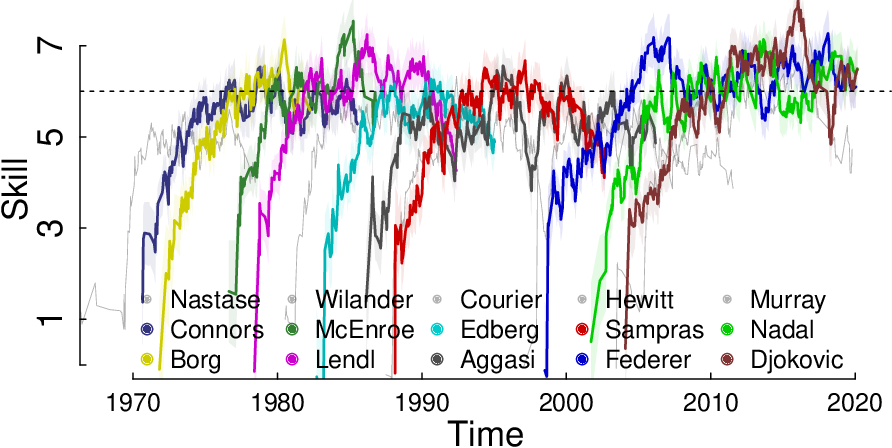
\includegraphics[page={1},width=.8\linewidth]{figures/atp_trueskill}
  \caption{ATP skill estimates using the TrueSkill model.}
  \label{atp_trueskill}
\end{figure}


\subsection{Gaussian product}\label{multiplicacion_normales}

The problem we must solve is:
\begin{equation}
 \int \N(x|\mu_1,\sigma_1^2)\N(x|\mu_2,\sigma_2^2) dx
\end{equation}
%
By definition,
\begin{equation}
\begin{split}
 \N(x|y,\beta^2)\N(x|\mu,\sigma^2) & = \frac{1}{\sqrt{2\pi}\sigma_1}e^{-\frac{(x-\mu_1)^2}{2\sigma_1^2}} \frac{1}{\sqrt{2\pi}\sigma_2}e^{-\frac{(x-\mu_2)^2}{2\sigma_2^2}}  \\
 & = \frac{1}{2\pi\sigma_1\sigma_2}\text{exp}\Bigg(-\underbrace{\left( \frac{(x-\mu_1)^2}{2\sigma_1^2} + \frac{(x-\mu_2)^2}{2\sigma_2^2} \right)}_{\theta} \Bigg)
\end{split}
\end{equation}
%
Then,
\begin{equation}
 \theta = \frac{\sigma_2^2(x^2 + \mu_1^2 - 2x\mu_1) + \sigma_1^2(x^2 + \mu_2^2 - 2x\mu_2) }{2\sigma_1^2\sigma_2^2}
\end{equation}
%
We expand and reorder the factors by powers of $x$
\begin{equation}
 \frac{(\sigma_1^2 + \sigma_2^2) x^2 - (2\mu_1\sigma_2^2 + 2\mu_2\sigma_1^2) x + (\mu_1^2\sigma_2^2 + \mu_2^2\sigma_1^2)}{2\sigma_1^2\sigma_2^2}
\end{equation}
%
We divide the numerator and denominator by the factor of $x^2$
\begin{equation}
 \frac{x^2 - 2\frac{(\mu_1\sigma_2^2 + \mu_2\sigma_1^2)}{(\sigma_1^2 + \sigma_2^2) } x + \frac{(\mu_1^2\sigma_2^2 + \mu_2^2\sigma_1^2)}{(\sigma_1^2 + \sigma_2^2) }}{2\frac{\sigma_1^2\sigma_2^2}{(\sigma_1^2 + \sigma_2^2)}}
\end{equation}
%
This equation is quadratic in x, and is therefore proportional to a Gaussian density function with standard deviation
\begin{equation}
\sigma_{\times} = \sqrt{\frac{\sigma_1^2\sigma_2^2}{\sigma_1^2+\sigma_2^2}}
\end{equation}
%
and mean
\begin{equation}
 \mu_{\times} = \frac{(\mu_1\sigma_2^2 + \mu_2\sigma_1^2)}{(\sigma_1^2 + \sigma_2^2) }
\end{equation}
%
Since a term $\varepsilon = 0$ can be added to complete the square in $\theta$, this proof is sufficient when no normalization is needed. 

%
\begin{equation}
 \varepsilon = \frac{\mu_{\times}^2-\mu_{\times}^2}{2\sigma_{\times}^2} = 0
\end{equation}
%
By adding this term to $\theta$ we obtain
\begin{equation}
 \theta = \frac{x^2 - 2\mu_{\times}x + \mu_{\times}^2 }{2\sigma_{\times}^2} + \underbrace{\frac{ \frac{(\mu_1^2\sigma_2^2 + \mu_2^2\sigma_1^2)}{(\sigma_1^2 + \sigma_2^2) } - \mu_{\times}^2}{2\sigma_{\times}^2}}_{\varphi}
\end{equation}
%
Reorganizing $\varphi$
\begin{equation}
\begin{split}
\varphi & = \frac{\frac{(\mu_1^2\sigma_2^2 + \mu_2^2\sigma_1^2)}{(\sigma_1^2 + \sigma_2^2) } - \left(\frac{(\mu_1\sigma_2^2 + \mu_2\sigma_1^2)}{(\sigma_1^2 + \sigma_2^2) }\right)^2 }{2\frac{\sigma_1^2\sigma_2^2}{\sigma_1^2+\sigma_2^2}}  \\
& = \frac{(\sigma_1^2 + \sigma_2^2)(\mu_1^2\sigma_2^2 + \mu_2^2\sigma_1^2) - (\mu_1\sigma_2^2 + \mu_2\sigma_1^2)^2}{\sigma_1^2 + \sigma_2^2}\frac{1}{2\sigma_1^2\sigma_2^2} \\[0.3cm]
& = \frac{(\mu_1^2\sigma_1^2\sigma_2^2 + \cancel{\mu_2^2\sigma_1^4} + \bcancel{\mu_1^2\sigma_2^4} + \mu_2^2\sigma_1^2\sigma_2^2) - (\bcancel{\mu_1^2\sigma_2^4} + 2\mu_1\mu_2\sigma_1^2\sigma_2^2 + \cancel{\mu_2^2\sigma_1^4} )}{\sigma_1^2 + \sigma_2^2}  \frac{1}{2\sigma_1^2\sigma_2^2} \\[0.3cm]
& = \frac{(\sigma_1^2\sigma_2^2)(\mu_1^2 + \mu_2^2 - 2\mu_1\mu_2)}{\sigma_1^2 + \sigma_2^2}\frac{1}{2\sigma_1^2\sigma_2^2} = \frac{\mu_1^2 + \mu_2^2 - 2\mu_1\mu_2}{2(\sigma_1^2 + \sigma_2^2)} = \frac{(\mu_1 - \mu_2)^2}{2(\sigma_1^2 + \sigma_2^2)}
\end{split}
\end{equation}
%
Then,
\begin{equation}
 \theta = \frac{(x-\mu_{\times})^2}{2\sigma_{\times}^2} + \frac{(\mu_1 - \mu_2)^2}{2(\sigma_1^2 + \sigma_2^2)}
\end{equation}
%
Putting $\theta$ in place
\begin{equation}
\begin{split}
 \N(x|y,\beta^2)\N(x|\mu,\sigma^2) & = \frac{1}{2\pi\sigma_1\sigma_2}\text{exp}\Bigg(-\underbrace{\left( \frac{(x-\mu_{\times})^2}{2\sigma_{\times}^2} + \frac{(\mu_1 - \mu_2)^2}{2(\sigma_1^2 + \sigma_2^2)} \right)}_{\theta} \Bigg) \\
 & = \frac{1}{2\pi\sigma_1\sigma_2}\text{exp}\left(  - \frac{(x-\mu_{\times})^2}{2\sigma_{\times}^2} \right) \text{exp} \left( - \frac{(\mu_1 - \mu_2)^2}{2(\sigma_1^2 + \sigma_2^2)} \right)
\end{split}
\end{equation}
%
Multiplying by $\sigma_{\times}\sigma_{\times}^{-1}$
\begin{equation}
\overbrace{\frac{\cancel{\sigma_1\sigma_2}}{\sqrt{\sigma_1^2+\sigma_2^2}}}^{\sigma_{\times}} \frac{1}{\sigma_{\times}} \frac{1}{2\pi\cancel{\sigma_1\sigma_2}}\text{exp}\left(  - \frac{(x-\mu_{\times})^2}{2\sigma_{\times}^2} \right) \text{exp} \left( - \frac{(\mu_1 - \mu_2)^2}{2(\sigma_1^2 + \sigma_2^2)} \right)
\end{equation}
%
Then,
\begin{equation}
 \frac{1}{\sqrt{2\pi}\sigma_{\times}}\text{exp}\left(  - \frac{(x-\mu_{\times})^2}{2\sigma_{\times}^2} \right) \frac{1}{\sqrt{2\pi(\sigma_1^2+\sigma_2^2)}} \text{exp} \left( - \frac{(\mu_1 - \mu_2)^2}{2(\sigma_1^2 + \sigma_2^2)} \right)
\end{equation}
%
Going back to the integral
\begin{equation}
\begin{split}
I & = \int \N(x|\mu_{\times},\sigma_{\times}^2) \overbrace{\N(\mu_1|\mu_2,\sigma_1^2 + \sigma_2^2)}^{\text{Scalar magnitude independent of x}} dx \\[0.3cm]
& = \N(\mu_1|\mu_2,\sigma_1^2 + \sigma_2^2) \underbrace{\int \N(x|\mu_{\times},\sigma_{\times}^2)  dx}_{\text{Integrates to 1}} \\
& = \N(\mu_1|\mu_2,\sigma_1^2 + \sigma_2^2)
\end{split}
\end{equation}

\subsection{Sum of Gaussians}\label{suma_normales_induccion}

Proof by induction,
\paragraph{Base case}
%
\begin{equation}
\begin{split}
 P(1) := \int \delta(t_1 = x_1) \N(x_1|\mu_1,\sigma_1^2) dx_1 = \N(t_1|\mu_1,\sigma_1^2)
\end{split}
\end{equation}
%
The proposition $P(1)$ is true given the properties of the delta Dirac function. 
%
\begin{equation}\label{eq:induccion_2}
\begin{split}
P(2) & := \iint \delta(t_2 = x_1 + x_2) \N(x_1|\mu_1, \sigma_1^2)\N(x_2|\mu_2, \sigma_2^2) dx_1dx_2 \\
 & \overset{\ref{eq:induccion_2}.1}{=} \int \N(x_1|\mu_1, \sigma_1^2) \N(t_2 - x_1|\mu_2, \sigma_2^2) dx_1   \\
 & \overset{\ref{eq:induccion_2}.2}{=} \int \N(x_1|\mu_1, \sigma_1^2) \N(x_1|t_2 - \mu_2, \sigma_2^2) dx_1 \\
 & \overset{*}{=} \int \underbrace{N(t_2|\mu_1+\mu_2,\sigma_1^2 + \sigma_2^2)}_{\text{const.}} \underbrace{\N(x_1|\mu_{*},\sigma_{*}^2) dx_1}_{1} \\
 & = \N(t_2|\mu_1+\mu_2,\sigma_1^2 + \sigma_2^2)
\end{split}
\end{equation}
where $\overset{\ref{eq:induccion_2}.1}{=}$ is valid for the properties of the dirac delta function, $\overset{\ref{eq:induccion_2}.2}{=}$ is valid for the symmetry of the Gaussians, and $\overset{*}{=}$ is valid by de proof at Section~\ref{multiplicacion_normales}. 
Therefore, $P(2)$ is valid. 

\paragraph{Inductive step} $P(n) \Rightarrow P(n+1)$

Given,
\begin{equation}
 P(n) :=\int \dots \int \delta(t_n= \sum_{i=1}^n x_i ) \left( \prod_{i=1}^n \N(x_i|\mu_i,\sigma_i^2) \right) dx_1 \dots dx_n = \N(t|\sum_{i=1}^n \mu_i,\sum_{i=1}^n \sigma_i^2 )
\end{equation}
%
We want to see that $P(n+1)$ is valid. 
%
\begin{equation}
 P(n+1) := \int \dots \int \delta(t_{n+1}=x_{n+1} + \sum_{i=1}^{n} x_i ) \left( \prod_{i=1}^{n} \N(x_i|\mu_i,\sigma_i^2) \right) \N(x_{n+1}|\mu_{n+1},\sigma_{n+1}^2) dx_1 \dots dx_{n} dx_{n+1}
\end{equation}
%
By independence
\begin{equation}
 \int \N(x_{n+1}|\mu_{n+1},\sigma_{n+1}^2) \left( \int \dots \int \delta(t_{n+1}= x_{n+1} + \sum_{i=1}^{n} x_i ) \left( \prod_{i=1}^{n} \N(x_i|\mu_i,\sigma_i^2) \right)  dx_1 \dots dx_{n}\right) dx_{n+1}
\end{equation}
%
By inductive hypothesis
\begin{equation}
 \int \N(x_{n+1}|\mu_{n+1},\sigma_{n+1}^2) \N(t_{n+1}-x_{n+1}|\sum_{i=1}^n \mu_i,\sum_{i=1}^n \sigma_i^2) dx_{n+1}
\end{equation}
%
By de proof of Section~\ref{multiplicacion_normales}
\begin{equation}
  \N(t_{n+1}|\mu_{n+1}+\sum_{i=1}^{n} \mu_i,\sigma_{n+1}^2 \sum_{i=1}^n \sigma_i^2) dx_{n+1}
\end{equation}
%
Therefore, $P(n+1)$ is valid

\subsection{A Gaussian multiplied by an cumulative Gaussian.}

We want to solve the integral
\begin{equation}
 f(x) = \int \N(y;\mu_1,\sigma_1^2)\Phi(y+x;\mu_2,\sigma_2^2) dy
\end{equation}
%
To do so, we take the derivative of the function $\frac{\partial}{\partial x}f(x) = \theta(x)$,
\begin{equation}
 \theta(x) = \frac{\partial}{\partial x}\int \N(y;\mu_1,\sigma_1^2)\Phi(y+x|\mu_2,\sigma_2^2) dy
\end{equation}
%
\begin{equation}
 \theta(x) = \int \N(y|\mu_1,\sigma_1^2)\frac{\partial}{\partial x}\Phi(y+x|\mu_2,\sigma_2^2) dy
\end{equation}
%
The derivative of $\Phi$ is indeed a Gaussian,
\begin{equation}
\begin{split}
\theta(x) & = \int \N(y|\mu_1,\sigma_1^2)\N(y+x|\mu_2,\sigma_2^2) dy \\
& = \int \N(y|\mu_1,\sigma_1^2)\N(y|\mu_2-x,\sigma_2^2) dy
\end{split}
\end{equation}
%
By the proof at Section~\ref{multiplicacion_normales} we know
\begin{equation}
 \theta(x) = \N(\mu_1| \mu_2 - x, \sigma_1^2 + \sigma_2^2)
\end{equation}
%
By symmetry
\begin{equation}
 \theta(x) = \N(x| \mu_2 - \mu_1, \sigma_1^2 + \sigma_2^2)
\end{equation}
%
Returning to $f(x)$
\begin{equation}
 f(x) = \Phi(x| \mu_2 - \mu_1, \sigma_1^2 + \sigma_2^2)
\end{equation}

\subsection{Gaussian division}\label{sec:division_normales}

\begin{equation}
\kappa = \frac{\N(x|\mu_f,\sigma_f^2)}{\N(x|\mu_g,\sigma_g^2)} = \N(x|\mu_f,\sigma_f^2)\N(x|\mu_g,\sigma_g^2)^{-1}
\end{equation}
%
By definition
\begin{equation}
\begin{split}
\kappa & = \frac{1}{\sqrt{2\pi}\sigma_f}e^{-\left(\frac{(x-\mu_f)^2}{2\sigma_f^2}\right)} \left( \frac{1}{\sqrt{2\pi}\sigma_g}e^{-\left(\frac{(x-\mu_g)^2}{2\sigma_g^2}\right)} \right)^{-1} \\[0.3cm]
& = \frac{1}{\cancel{\sqrt{2\pi}}\sigma_f}e^{-\left(\frac{(x-\mu_f)^2}{2\sigma_f^2}\right)} \frac{\cancel{\sqrt{2\pi}}\sigma_g}{1} e^{\left(\frac{(x-\mu_g)^2}{2\sigma_g^2}\right)} \\[0.3cm]
& = \frac{\sigma_g}{\sigma_f}\text{exp}\Bigg(-\underbrace{\Big(\frac{(x-\mu_f)^2}{2\sigma_f^2} - \frac{(x-\mu_g)^2}{2\sigma_g^2}\Big)}_{\theta}\Bigg)
\end{split}
\end{equation}
%
Reorganizing $\theta$
\begin{equation}
\begin{split}
 \theta & = \frac{(x-\mu_f)^2}{2\sigma_f^2} - \frac{(x-\mu_g)^2}{2\sigma_g^2} = \frac{\sigma_g^2(x-\mu_f)^2 - \sigma_f^2(x-\mu_g)^2}{2\sigma_f^2\sigma_g^2} \\[0.3cm]
 & = \frac{\sigma_g^2(x^2+\mu_f^2-2\mu_fx) - \sigma_f^2(x^2+\mu_g^2-2\mu_gx)}{2\sigma_f^2\sigma_g^2}
\end{split}
\end{equation}
%
We expand and sort terms based on $x$,
%
\begin{equation}
\begin{split}
 \theta & = \left((\sigma_g^2 - \sigma_f^2)x^2 - 2(\sigma_g^2\mu_f - \sigma_f^2\mu_g)x + (\sigma_g^2\mu_f^2 - \sigma_f^2\mu_g^2 )\right) \frac{1}{2\sigma_f^2\sigma_g^2} \\[0.3cm]
 & = \left(x^2 - \frac{2(\sigma_g^2\mu_f - \sigma_f^2\mu_g)}{(\sigma_g^2 - \sigma_f^2)}x + \frac{(\sigma_g^2\mu_f^2 - \sigma_f^2\mu_g^2 )}{(\sigma_g^2 - \sigma_f^2)}\right) \frac{(\sigma_g^2 - \sigma_f^2)}{2\sigma_f^2\sigma_g^2}
\end{split}
\end{equation}
%
This is quadratic in $x$. Since a term $\varepsilon=0$ independent of $x$ can be added to complete the square in $\theta$, this test is sufficient to determine the mean and variance when it is not necessary to normalize. 

%
\begin{equation}
 \sigma_{\div} = \sqrt{\frac{\sigma_f^2\sigma_g^2}{(\sigma_g^2 - \sigma_f^2)}}
\end{equation}
%
\begin{equation}
 \mu_{\div} = \frac{(\sigma_g^2\mu_f - \sigma_f^2\mu_g)}{(\sigma_g^2 - \sigma_f^2)}
\end{equation}
%
adding $\varepsilon = \frac{\mu_{\div}^2-\mu_{\div}^2}{2\sigma_{\div}^2} = 0$
\begin{equation}
\theta = \frac{x^2 - 2\mu_{\div}x + \mu_{\div}^2 }{2\sigma_{\div}^2} + \underbrace{ \frac{ \frac{(\sigma_g^2\mu_f^2 - \sigma_f^2\mu_g^2)}{(\sigma_g^2 - \sigma_f^2)} - \mu_{\div}^2 }{2\sigma_{\div}^2} }_{\varphi}
\end{equation}

Reorganizing $\varphi$
\begin{equation}
\begin{split}
 \varphi & = \left( \frac{(\sigma_g^2\mu_f^2 - \sigma_f^2\mu_g^2)}{(\sigma_g^2 - \sigma_f^2)} - \left(\frac{(\sigma_g^2\mu_f - \sigma_f^2\mu_g)}{(\sigma_g^2 - \sigma_f^2)} \right)^2 \right) \frac{(\sigma_g^2 - \sigma_f^2)}{2\sigma_f^2\sigma_g^2} \\[0.3cm]
 & = \left((\sigma_g^2\mu_f^2 - \sigma_f^2\mu_g^2)(\sigma_g^2 - \sigma_f^2) - \left((\sigma_g^2\mu_f - \sigma_f^2\mu_g) \right)^2 \right) \frac{1}{2\sigma_f^2\sigma_g^2(\sigma_g^2 - \sigma_f^2)} \\[0.3cm]
 & =  \left( \cancel{\sigma_g^4\mu_f^2} - \sigma_f^2\sigma_g^2\mu_f^2 - \sigma_f^2\sigma_g^2\mu_g^2 + \bcancel{\sigma_f^4\mu_g^2} - (\cancel{\sigma_g^4\mu_f^2} + \bcancel{\sigma_f^4\mu_g^2 } - 2\sigma_f^2\sigma_g^2\mu_f\mu_g)\right) \frac{1}{2\sigma_f^2\sigma_g^2(\sigma_g^2 - \sigma_f^2)}
 \end{split}
\end{equation}
%
Canceling $\sigma_f^2\sigma_g^2$
\begin{equation}
 \varphi = \frac{- \mu_g^2 - \mu_f^2 + 2\mu_f\mu_g}{2(\sigma_g^2 - \sigma_f^2)} = \frac{- (\mu_g - \mu_f)^2}{2(\sigma_g^2 - \sigma_f^2)}
\end{equation}
%
Then $\theta$
\begin{equation}
 \theta = \frac{(x - \mu_{\div})^2}{2\sigma_{\div}^2} - \frac{(\mu_g - \mu_f)^2)}{2(\sigma_g^2 - \sigma_f^2)}
\end{equation}

Returning to the original expression
\begin{equation}
\begin{split}
 \kappa & = \frac{\sigma_g}{\sigma_f}  \, \text{exp}\left(- \frac{(x - \mu_{\div})^2}{2\sigma_{\div}^2} + \frac{(\mu_g - \mu_f)^2)}{2(\sigma_g^2 - \sigma_f^2)}  \right)\\[0.3cm]
 & = \frac{\sigma_g}{\sigma_f} \, \text{exp}\left({-\frac{(x - \mu_{\div})^2}{2\sigma_{\div}^2}}\right) \, \text{exp}\left({\frac{(\mu_g - \mu_f)^2)}{2(\sigma_g^2 - \sigma_f^2)}}\right)
\end{split}
\end{equation}

Multiplying by $\frac{\sqrt{2\pi}}{\sqrt{2\pi}}\frac{\sigma_{\div}}{\sigma_{\div}}\frac{\sqrt{\sigma_g^2 - \sigma_f^2}}{\sqrt{\sigma_g^2 - \sigma_f^2}}=1$,
\begin{equation}
\begin{split}
 \kappa & =  \frac{1}{\sqrt{2\pi}\sigma_{\div}} \, e^{-\frac{(x - \mu_{\div})^2}{2\sigma_{\div}^2}} \, \left( \frac
 {1}{\sqrt{2\pi(\sigma_g^2 - \sigma_f^2)} } e^{-\frac{(\mu_g - \mu_f)^2)}{2(\sigma_g^2 - \sigma_f^2)}} \right)^{-1} \, \frac{\sigma_{\div}}{\sqrt{\sigma_g^2 - \sigma_f^2}}\frac{\sigma_g}{\sigma_f}\\[0.3cm]
 & = \frac{\N\left(x| \mu_{\div},\sigma_{\div}\right)}{\N\left(\mu_g|\mu_f,\sigma_g^2-\sigma_f^2\right)} \frac{\sigma_g^2}{\sigma_g^2 - \sigma_f^2}
\end{split}
\end{equation}




%% -----------------------------------------------------------------------------

\end{document}
